\documentclass{IEEEtran}
\usepackage{xcolor}
\usepackage{cite}
\usepackage{amsmath,amssymb,amsfonts}
\usepackage{graphicx}
\usepackage{textcomp,nicefrac}
\usepackage[pdfa]{hyperref}
\usepackage[a-2b,mathxmp]{pdfx}\usepackage[utf8]{inputenc}
\usepackage[english]{babel}
\usepackage[T1]{fontenc}
\usepackage{setspace}
\usepackage{amsfonts}
\usepackage{harmony}
\usepackage{graphicx}
\graphicspath{ {./images/} }
\usepackage{subcaption}
\usepackage{float}
\usepackage{caption}
\usepackage{makecell}
\usepackage{array}
\usepackage{booktabs}
\usepackage{verbatim}
\usepackage{amsmath}
\usepackage{booktabs}

\newcommand{\Cels}{^{\circ}C}
\newcommand{\half}{\frac{1}{2}}
\newcommand{\measure}[2]{\ensuremath{#1 \, \mathrm{#2}}}

\def\BibTeX{{\rm B\kern-.05em{\sc i\kern-.025em b}\kern-.08em T\kern-.1667em\lower.7ex\hbox{E}\kern-.125emX}}

\markboth{IEEE TRANSACTIONS ON NUCLEAR SCIENCE, VOL. XX, NO. XX, XXXX 2025}
{Author \MakeLowercase{\textit{et al.}}: Preparation of Papers for	Review by the \textsc{IEEE Transactions on Nuclear Science} \newline (Jan 2025)}

\begin{document}
	
	\title{An integrated biasing power supply, control and acquisition system for large Langmuir probe arrays in cold plasmas}
	\author{M. Bevilacqua$^{1,3}$, R. Cavazzana$^{1}$, S. Spagnolo$^{1,2}$, M. Spolaore$^{1,2}$, G. Manduchi$^{1}$, N. Ferron$^{1}$, B. Segalini$^{1}$, F. Milan$^{4}$, R. Pasqualotto$^{1,2}$
		
		\thanks{$^1$Consorzio RFX (CNR, ENEA, INFN, Università di Padova, Acciaierie Venete SpA)}
		\thanks{$^2$ISTP - Istituto per la Scienza e Tecnologia dei Plasmi, Padova, Italy}
		\thanks{$^3$Centro Ricerche Fusione (CRF) – University of Padova, 35131 Padova, Italy}
		\thanks{$^4$ELAD srl - 33070 Caneva (PN), Italy}
	}
	\maketitle
	
	\begin{abstract}
		Large Langmuir probe arrays are widely employed in plasma diagnostics for fusion devices, where synchronized acquisition and scalable instrumentation architectures are required. A representative example is MITICA, the full-scale neutral beam injector prototype for ITER, which foresees more than 200 distributed electrostatic probe measurements along the beam line. This work presents EPICA, an integrated power supply, control, and data acquisition platform specifically developed to address the scalability limitations of conventional Langmuir probe systems based on centralized laboratory instrumentation. Unlike traditional architectures, EPICA integrates the complete measurement chain, including probe bias generation, signal conditioning, acquisition, and processing, within distributed probe modules. This approach significantly reduces wiring complexity, eliminates the need for centralized bias supplies, and enables straightforward scaling to large probe arrays. The system is based on a modular architecture employing automotive-grade System-on-Module technology that combines FPGA fabric and ARM processing cores, enabling deterministic real-time control and data processing. A custom Linux distribution, integrated with the MARTe2 framework, provides supervisory control and data management, while synchronization is achieved through either a dedicated timing system or the Precision Time Protocol (PTP). The platform supports floating-potential, single-probe, and double-probe configurations and operates over plasma conditions relevant to MITICA. Experimental validation demonstrated compliance with the measurement requirements defined for MITICA operation, confirming the suitability of the proposed architecture for large-scale Langmuir probe diagnostics in fusion-relevant environments.
		
	\end{abstract}
	
	\begin{IEEEkeywords}
		Acquisition Systems, Analogue Electronics, Digital Electronics, FPGAs, Fusion, Langmuir Probes
	\end{IEEEkeywords}
	
	\section{Introduction} \label{secI}
	The characterization of plasma parameters is essential for understanding and optimizing plasma-based systems. Among the available diagnostic techniques, Langmuir probes are widely used because they provide direct access to key plasma properties, including electron density, electron temperature, plasma potential, and the electron energy distribution function \cite{Chen,Crowley}. These quantities are extracted from the probe current-voltage (I-V) characteristic, making Langmuir probes a versatile and cost-effective diagnostic tool across a broad range of plasma conditions. However, due to their intrusive nature and limited survivability in high-temperature environments, Langmuir probes are generally restricted to low-temperature plasmas or Scrape Off Layer (SOL), where the perturbation introduced by the probe remains acceptable and plasma parameters can be reliably inferred from the measured I-V characteristics.

Fig.~\ref{fig1} illustrates the general configuration of a Langmuir probe measurement system. The diagnostic principle is simple: a metallic electrode is inserted into the plasma, biased over a controlled voltage range, and the resulting current response is measured. In practice, the setup typically includes a programmable bias power supply and a data acquisition system for recording the I-V characteristic. Such systems are commonly implemented using commercial off-the-shelf (COTS) instrumentation, including four-quadrant power supplies and modular data acquisition platforms \cite{NI,CAEN,Kepco} and are well suited for applications involving a limited number of measurements (up to ten simultaneous measurements). However, when a large number of spatially distributed measurements is required, conventional architectures become increasingly difficult to scale. The resulting increase in system complexity, footprint, and cost limits their applicability in large-area plasma diagnostics.


\begin{figure}[t]
	\centering
	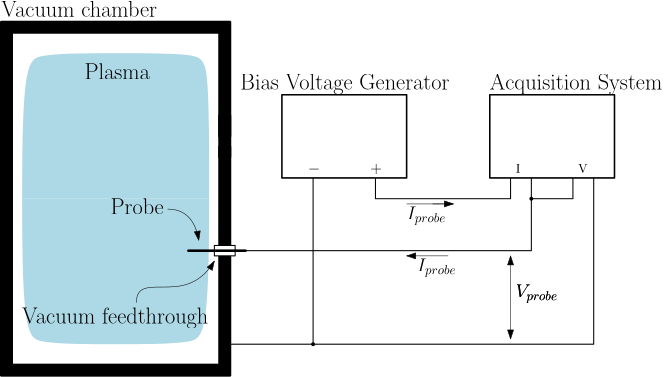
\includegraphics[width=3.4in]{lpms}
	\caption{General layout of a Langmuir probe acquisition system.}
	\label{fig1}
\end{figure}

A representative example of large-scale cold-plasma diagnostics is the Megavolt ITER Injector and Concept Advancement (MITICA), illustrated in Fig.~\ref{fig2}. MITICA is the full-scale prototype of the Neutral Beam Injector (NBI) for the International Thermonuclear Experimental Reactor (ITER) \cite{Toigo}. Installed at the PRIMA test facility in Padua, Italy, it is designed to demonstrate full-performance operation of the ITER neutral beam system, including the generation and acceleration of negative ion beams up to \measure{1}{MeV}. Plasma monitoring in MITICA relies on an extensive network of electrostatic probes distributed along the beam line, comprising a total of 212 measurement points located in the Neutralizer, Residual Ion Dump (RID), and Calorimeter. These diagnostics operate in multiple configurations, including Single and Double Langmuir Probe modes, and provide measurements of floating potential, electron temperature, plasma density, beam profiles, and secondary electron emission processes \cite{SPAGNOLO}. The large number of distributed measurements, together with the need for synchronized operation and flexible probe configurations, introduces significant challenges in terms of bias generation, data acquisition, and overall system scalability.



\begin{figure}[t]
	\centering
	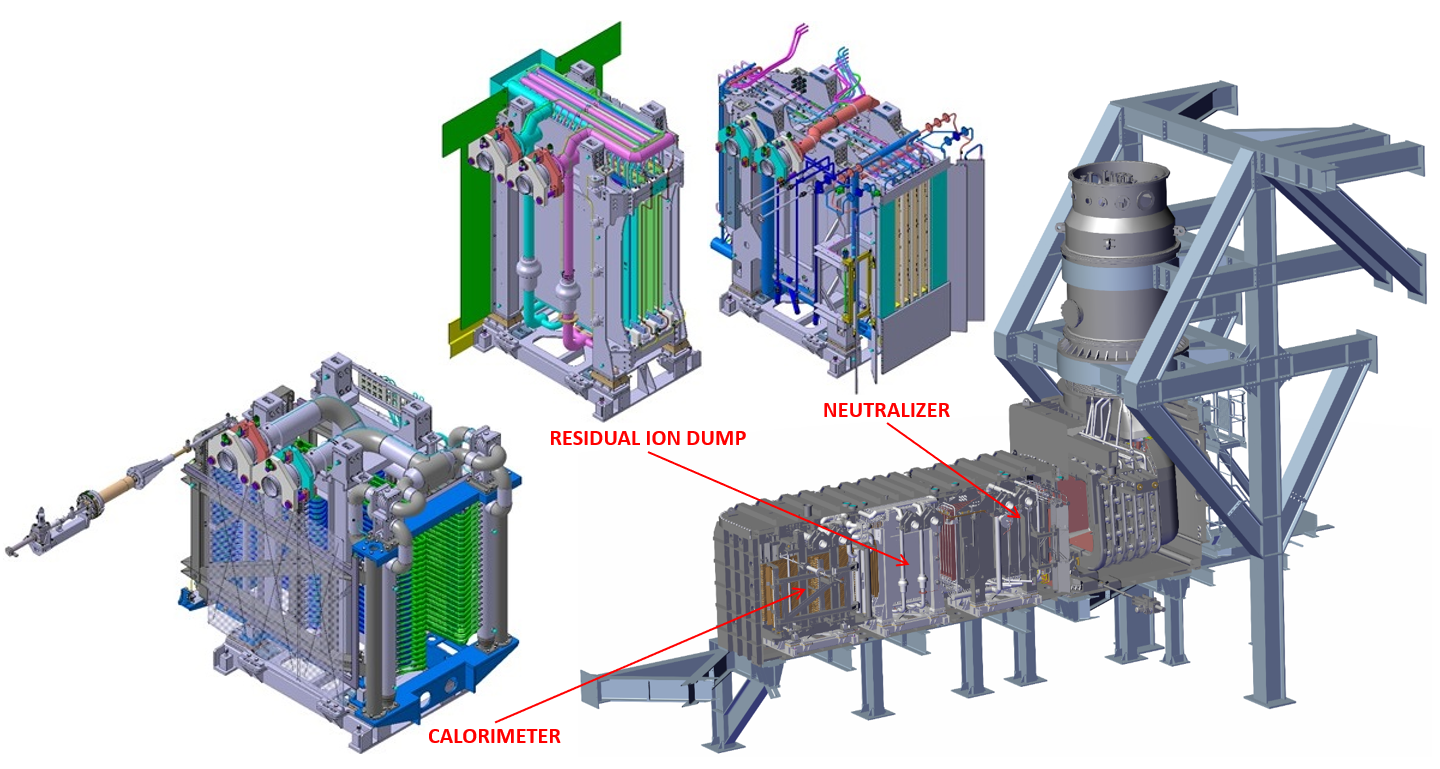
\includegraphics[width=3.4in]{MITICA3}
	\caption{MITICA design. The three components at the bottom of the schematic identifies the locations designated for probe installation.}
	\label{fig2}
\end{figure}

\begin{table}[t]
	\centering
	\footnotesize
	\renewcommand{\arraystretch}{1.5}
	\caption{Measurement ranges and relative resolution requirements.}
	\label{tab:meas_ranges}
	\begin{tabular}{c|c|c}
		\toprule
		\makecell{Measurement Range} & \makecell{Minimum \\resolution} & \makecell{Maximum residual \\r.m.s. noise} \\
		\midrule
		
		\multicolumn{3}{c}{\textit{Voltage measurements}} \\
		\midrule
		$\pm 100\,\mathrm{V}$ & $50\,\mathrm{mV}$ & $15\,\mathrm{mV}$ \\
		\midrule
		
		\multicolumn{3}{c}{\textit{Current measurements}} \\
		\midrule
		$\pm 1\,\mathrm{mA}$   & $0.5\,\mu\mathrm{A}$  & $0.15\,\mu\mathrm{A}$ \\
		$\pm 10\,\mathrm{mA}$  & $5\,\mu\mathrm{A}$    & $1.5\,\mu\mathrm{A}$ \\
		$\pm 100\,\mathrm{mA}$ & $50\,\mu\mathrm{A}$   & $15\,\mu\mathrm{A}$ \\
		$\pm 1\,\mathrm{A}$    & $500\,\mu\mathrm{A}$    & $150\,\mu\mathrm{A}$ \\
		\bottomrule
	\end{tabular}
\end{table}

Recent developments have addressed scalability limitations through the adoption of FPGA-based electronics. An example is the MAST-Upgrade Langmuir probe system, where dedicated control modules based on Xilinx Zynq devices provide arbitrary bias waveform generation and synchronized acquisition of voltage and current measurements from multiple probes \cite{Ryan}. Whereas this approach significantly improves scalability with respect to conventional laboratory instrumentation, the biasing and acquisition functions remain partially centralized and rely on multiplexed probe operation.

To address these challenges, this work presents EPICA (Electrostatic Probe Integrated Conditioning and Data Acquisition module), an integrated platform that combines power supply, control, and data acquisition functionalities for large Langmuir probe arrays. Unlike conventional systems based on centralized COTS instrumentation, EPICA embeds the probe biasing stage directly within each acquisition module. This approach improves scalability, reduces wiring complexity, and increases modularity, making the system better suited for high-density probe deployments.

EPICA is built on a high-performance hardware and software framework fully compatible with the ITER Control, Data Access and Communication (CODAC) system. The platform is designed to operate across a wide range of plasma conditions, covering electron densities from fractions of \measure{10^{15}}{m^{-3}} to \measure{10^{18}}{m^{-3}}, electron temperatures ranging from \measure{1}{eV} to \measure{10}{eV}, multiple probe configurations, and real-time data processing.

The proposed architecture supports synchronized operation across multiple distributed racks while satisfying the measurement resolution and noise requirements summarized in Table~\ref{tab:meas_ranges}. The requirements reported in Table~\ref{tab:meas_ranges} were derived from the expected plasma parameters and measurement accuracy targets defined for MITICA operation.

The main contributions of this work are threefold: (i) the development of a fully integrated probe-level biasing and acquisition module for high-density Langmuir probe arrays; (ii) a modular rack-based architecture scalable to large numbers of probes while maintaining synchronization; and (iii) a hardware and software implementation based on System-on-Module (SoM) technology and real-time frameworks enabling deterministic acquisition and processing in fusion-relevant plasma environments.

This paper is organized as follows. Section~\ref{secII} describes EPICA system architecture; Section~\ref{secIII} details the integrated polarization and acquisition module; Section~\ref{secIV} presents the software integration; Section~\ref{secV} reports the experimental validation; Section~\ref{secVI} discusses the results and Section~\ref{secVII} concludes the paper.
	
	\section{EPICA architecture} \label{secII}
	\begin{figure*}[t]
	\centering
	
	\subfloat[EPICA rack: from left to right: the power supply, the timing module, the control module and eight probe modules.]{
		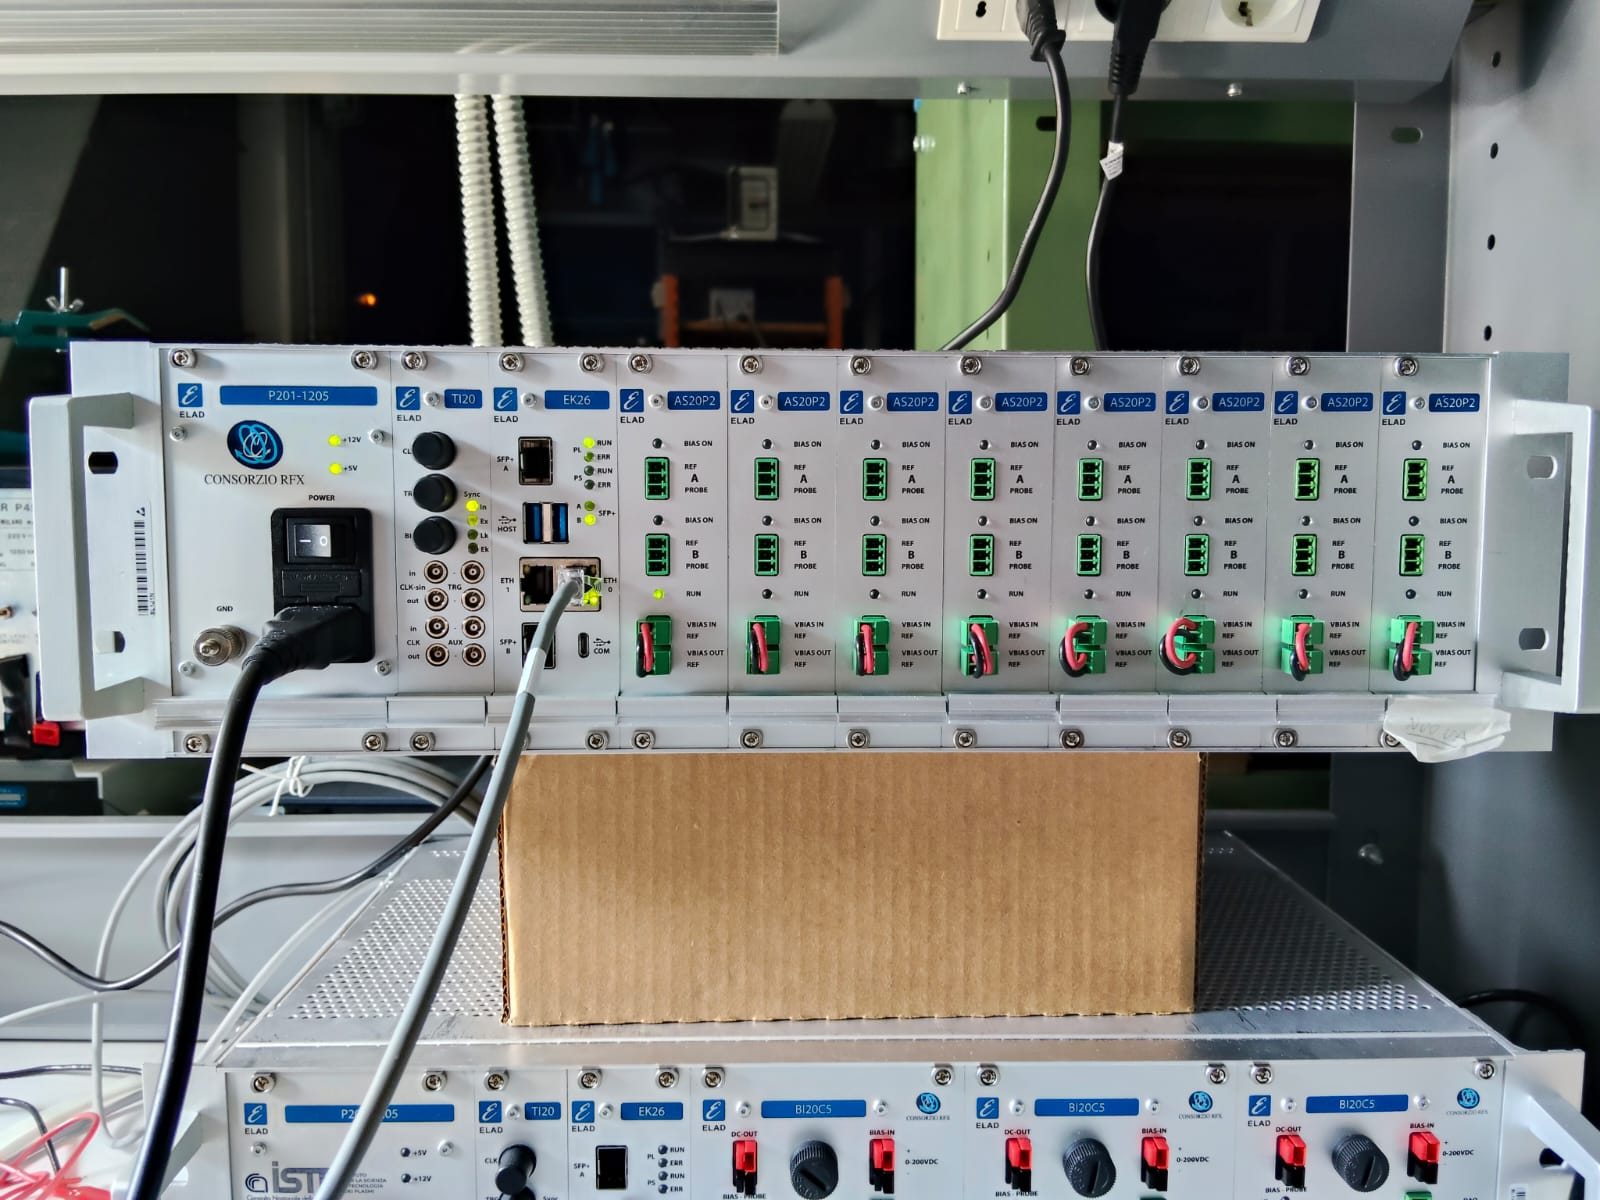
\includegraphics[width=3.2in]{epica}
		\label{fig3a}
	}
	\hfill
	\subfloat[Integrated probe management module, including biasing and signal conditioning stages.]{
		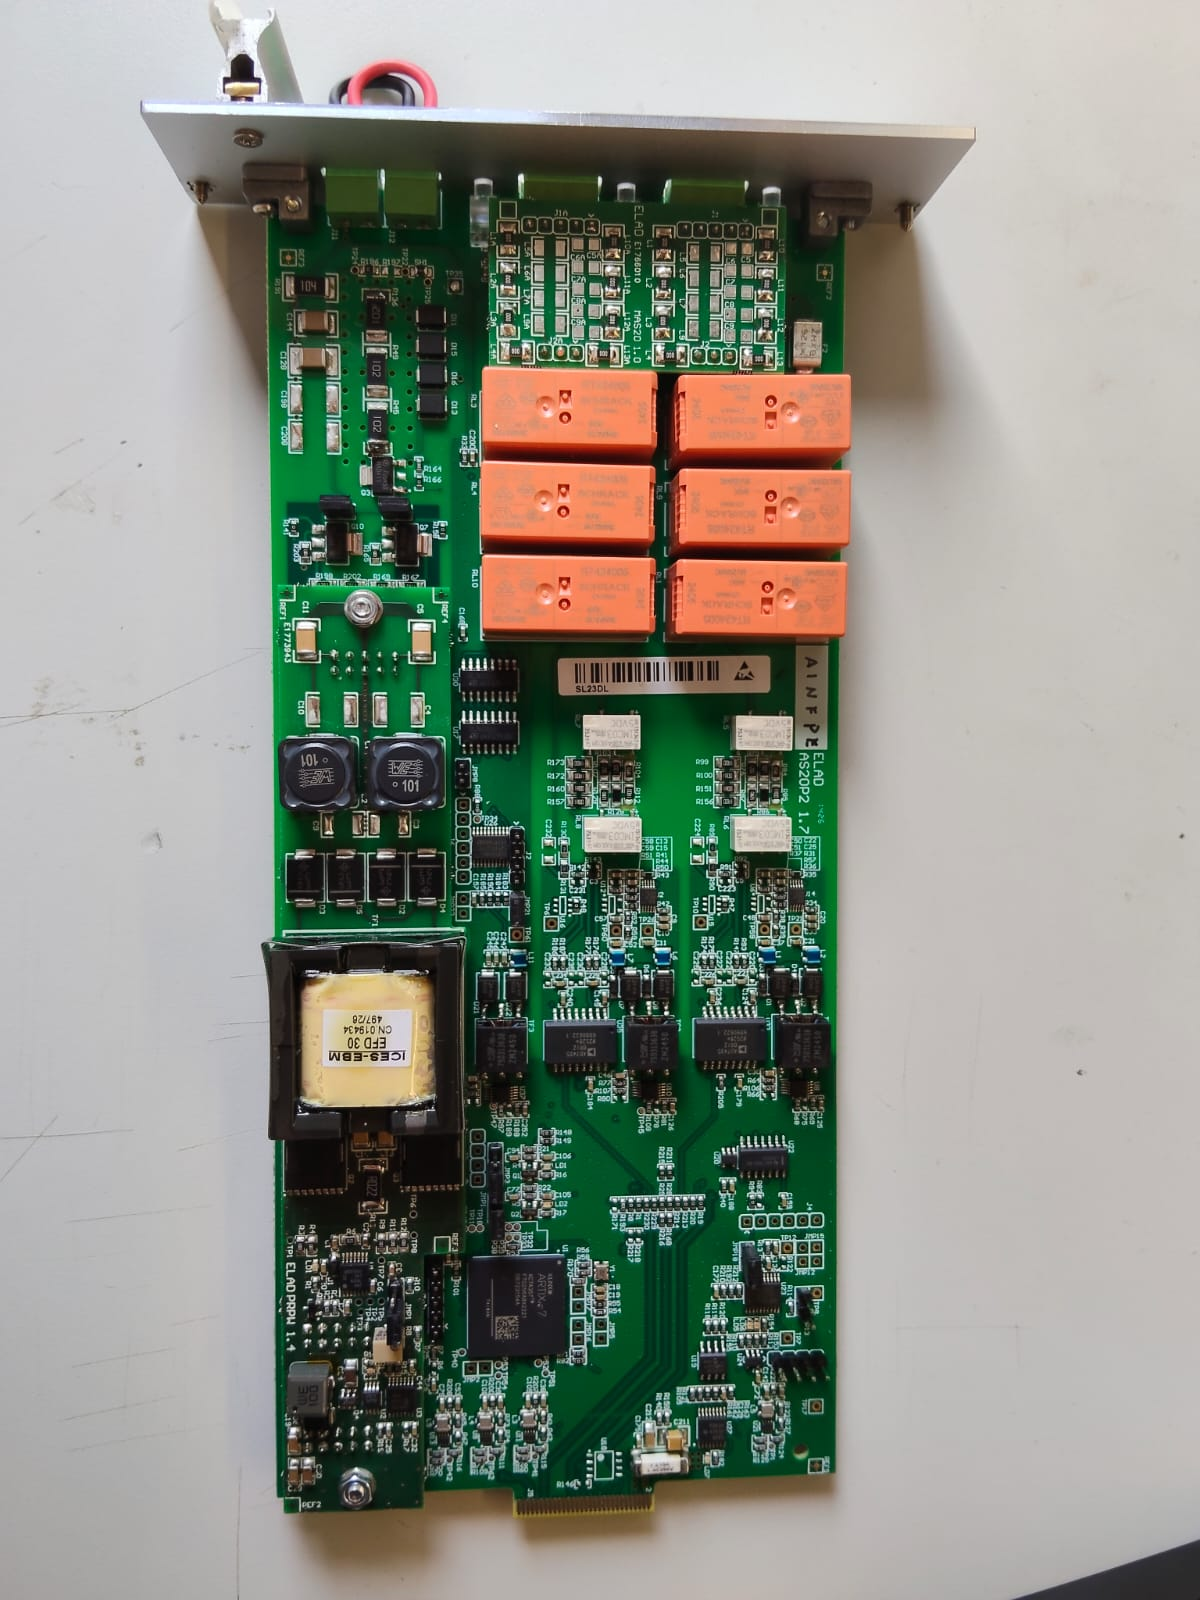
\includegraphics[width=2.3in,angle=90]{epica_module}
		\label{fig3b}
	}
	\vspace{0.5cm}
	\subfloat[Epica internal system overview.]{
		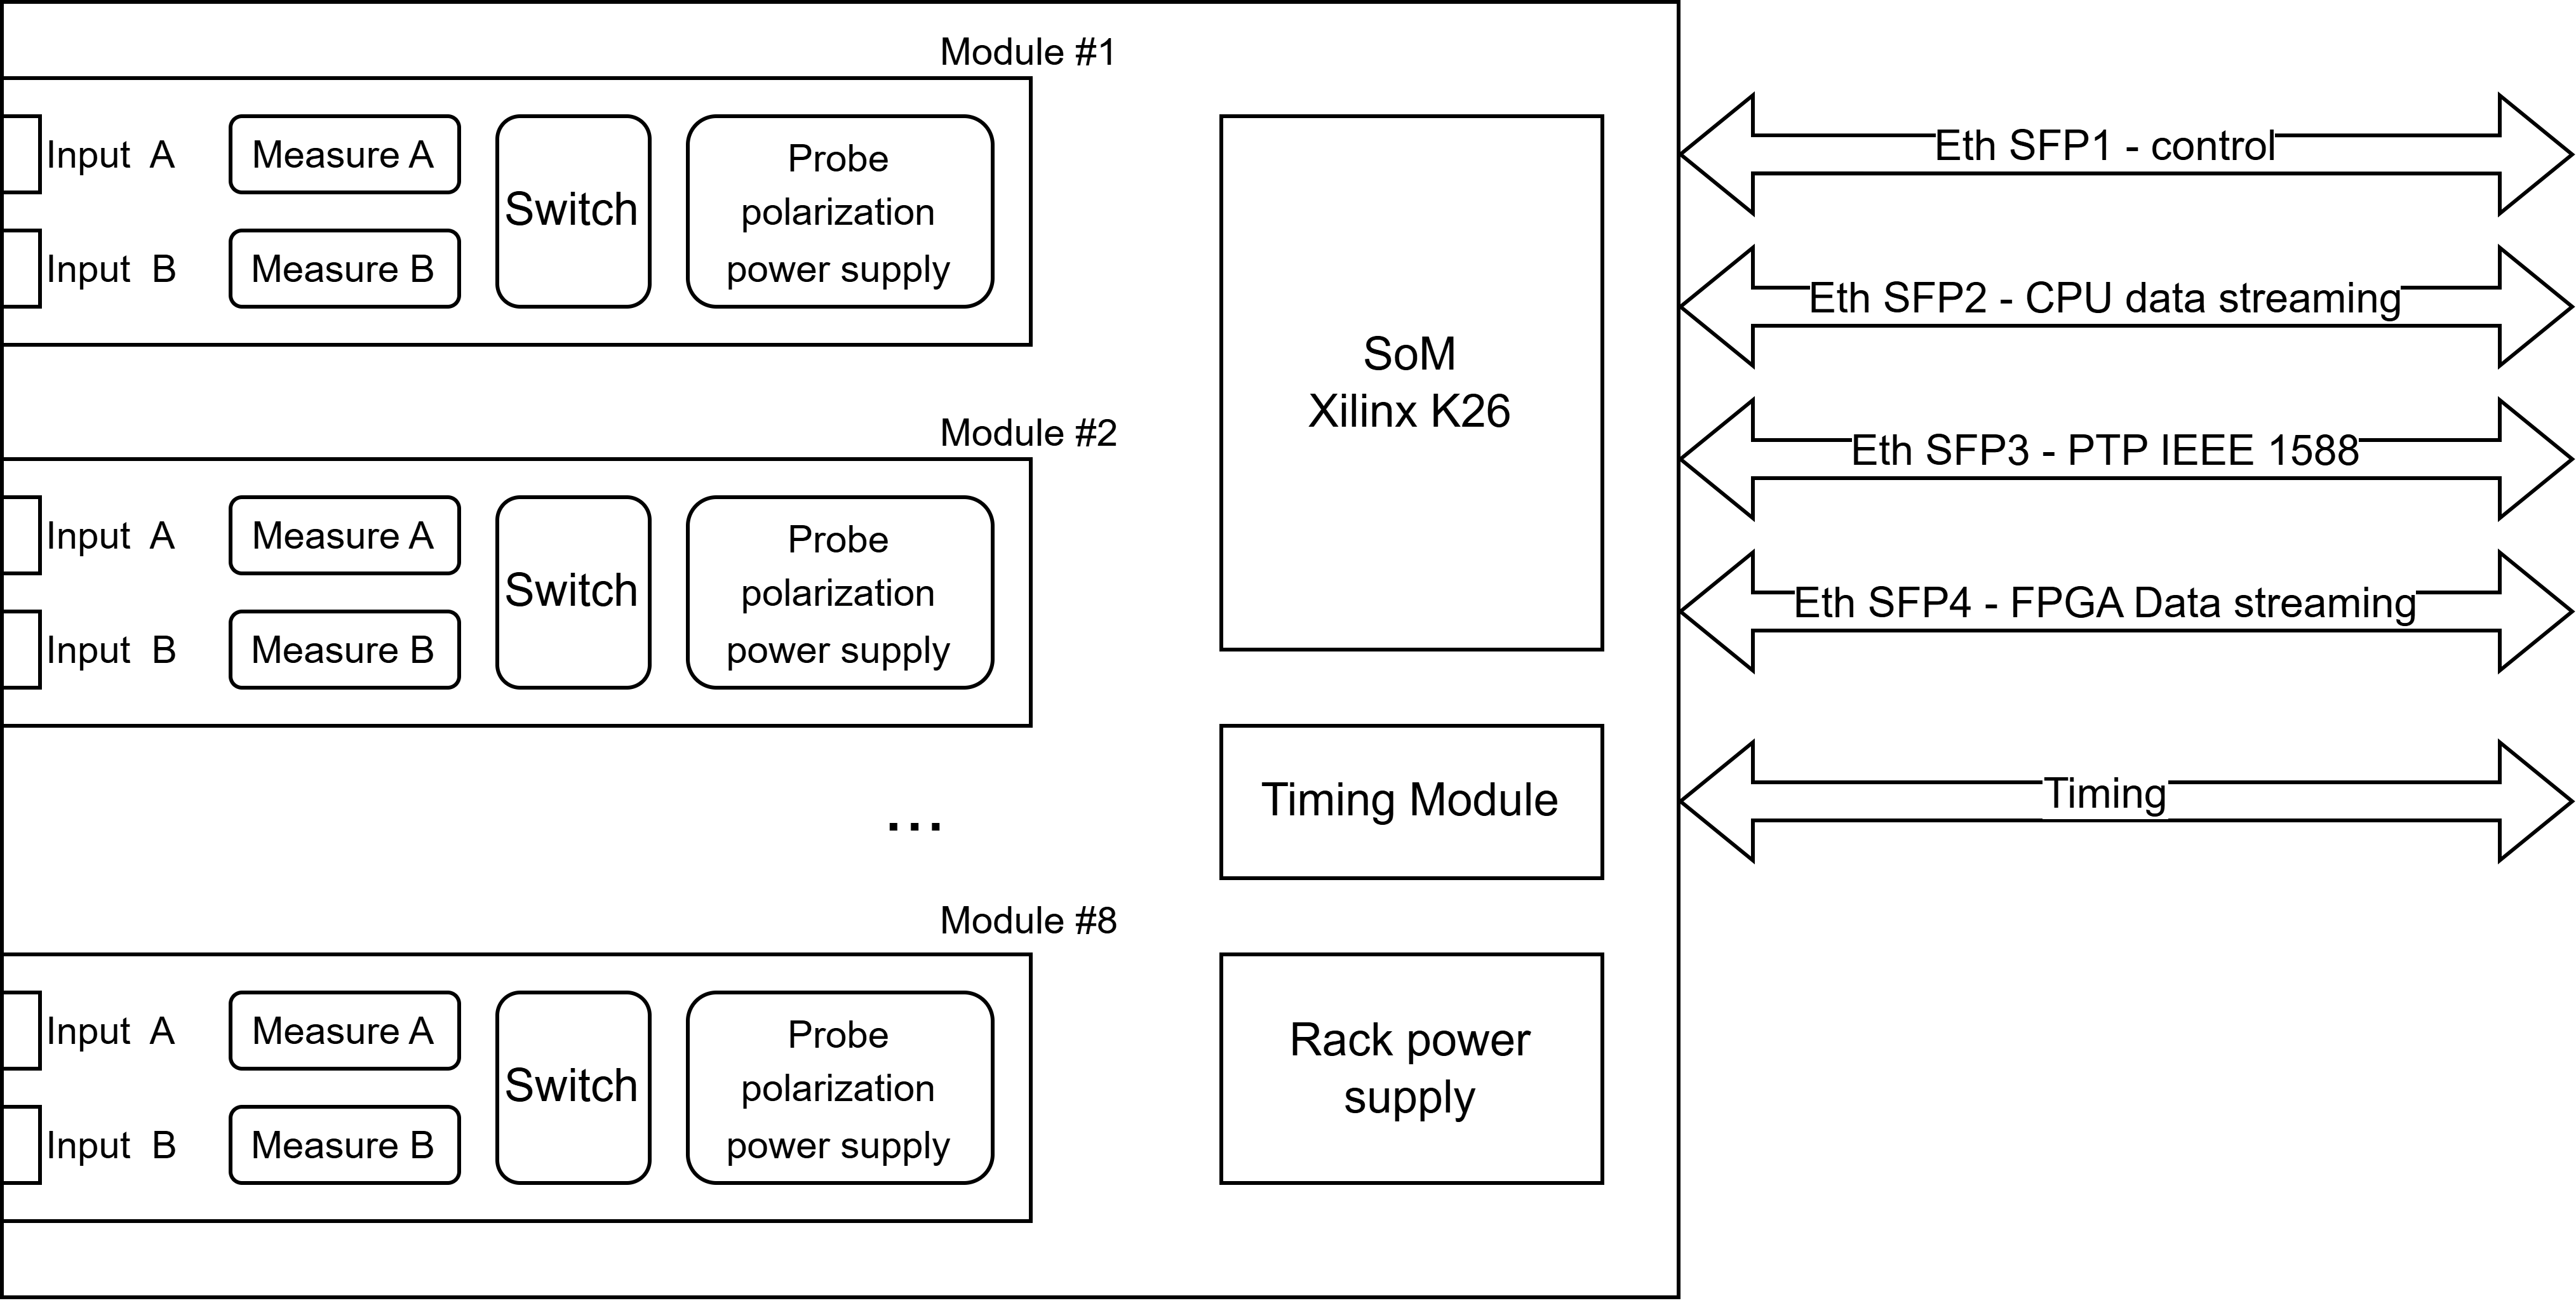
\includegraphics[width=4in]{epica_int4}
		\label{fig3c}
	}
	
	\caption{EPICA housing, probe management module and system overview.}
	\label{fig3}
\end{figure*}

Fig.~\ref{fig3a} shows the rack enclosure hosting the complete system, whereas Fig.~\ref{fig3c} illustrates the internal system overview. The platform supports up to 16 probes, arranged into eight electrically and functionally independent probe pairs. Each pair is managed by a dedicated acquisition and biasing module responsible for electrode polarization and signal acquisition. This modular organization enables straightforward system expansion while maintaining electrical isolation and operational flexibility, making EPICA suitable for a broad range of plasma diagnostics applications.

The system consists of four main subsystems: the power supply unit, the timing module, the controller module, and probe modules.

The power supply unit generates the primary \measure{5}{V} and \measure{12}{V} DC rails distributed throughout the system. Additional voltage levels required by individual subsystems are generated locally through dedicated DC/DC converters integrated within each module, ensuring proper electrical isolation both between modules and among different functional sections of the same module. This distributed power architecture also mitigates ground-loop effects.

The timing module provides the synchronization reference for both the controller and probe modules. It can operate either as a standalone timing source or be connected to an external master clock, enabling synchronization with other diagnostics and consistent temporal correlation of measurements. Alternatively, when Precision Time Protocol (PTP) synchronization is adopted, timing information is distributed through the Ethernet network, eliminating the need for a dedicated timing module. In this configuration, the PTP interface is implemented within the controller module.

To support integrated probe biasing, real-time data streaming and high-resolution acquisition, EPICA relies on a high-performance controller platform based on the KRIA K26 SoM \cite{KRIA}. The selected platform combines an FPGA with a quad-core ARM processor within the same chip, enabling tight integration between deterministic real-time control and high-throughput data processing.

Communication between modules is carried out using the back panel bus. It consists of Low Voltage Differential Signal (LVDS) rails for clock distribution and data exchange, and DC power rails for power transmission.

The system software is implemented using the MARTe2 \cite{manduchi} real-time framework, executed on the embedded processor to manage supervisory control, and communication tasks. Time-critical functions, including low-latency signal acquisition and preprocessing, are implemented within the FPGA. 

The probe modules implement the analog front-end electronics, probe bias generation, signal conditioning, and analog-to-digital conversion. Digitized measurements are transmitted to the controller via LVDS rails of the back panel bus for further processing, storage, and streaming.

Communication between EPICA and external systems is performed through Ethernet interfaces, available on the controller, as illustrated in Fig.~\ref{fig3c}, enabling simultaneous data streaming, synchronization, and integration with supervisory frameworks. In addition, a USB serial console is provided for system configuration, firmware deployment and debugging.
	
	\section{Integrated Polarization and Acquisition module} \label{secIII}
	Fig.~\ref{fig3b} shows the module managing the polarization, conditioning and acquisition of the probe signals. By embedding functionalities traditionally implemented through bulky laboratory equipment, as illustrated in Fig.~\ref{fig1}, the system significantly reduces spatial overhead and improves scalability for large arrays.

A key feature of the architecture is its ability to dynamically reconfigure both measurement range and probe measurement topology without requiring physical intervention at the instrumentation rack. 

To ensure robustness under harsh operating conditions, the plasma-facing circuitry is galvanically isolated from the digital processing electronics. This isolation strategy, carried out directly within the Analog to Digital Converter (ADC), protects low-voltage hardware while preserving signal integrity in the presence of high-voltage transients and electromagnetic interference (EMI).

\begin{figure*}[t]
	\centering
	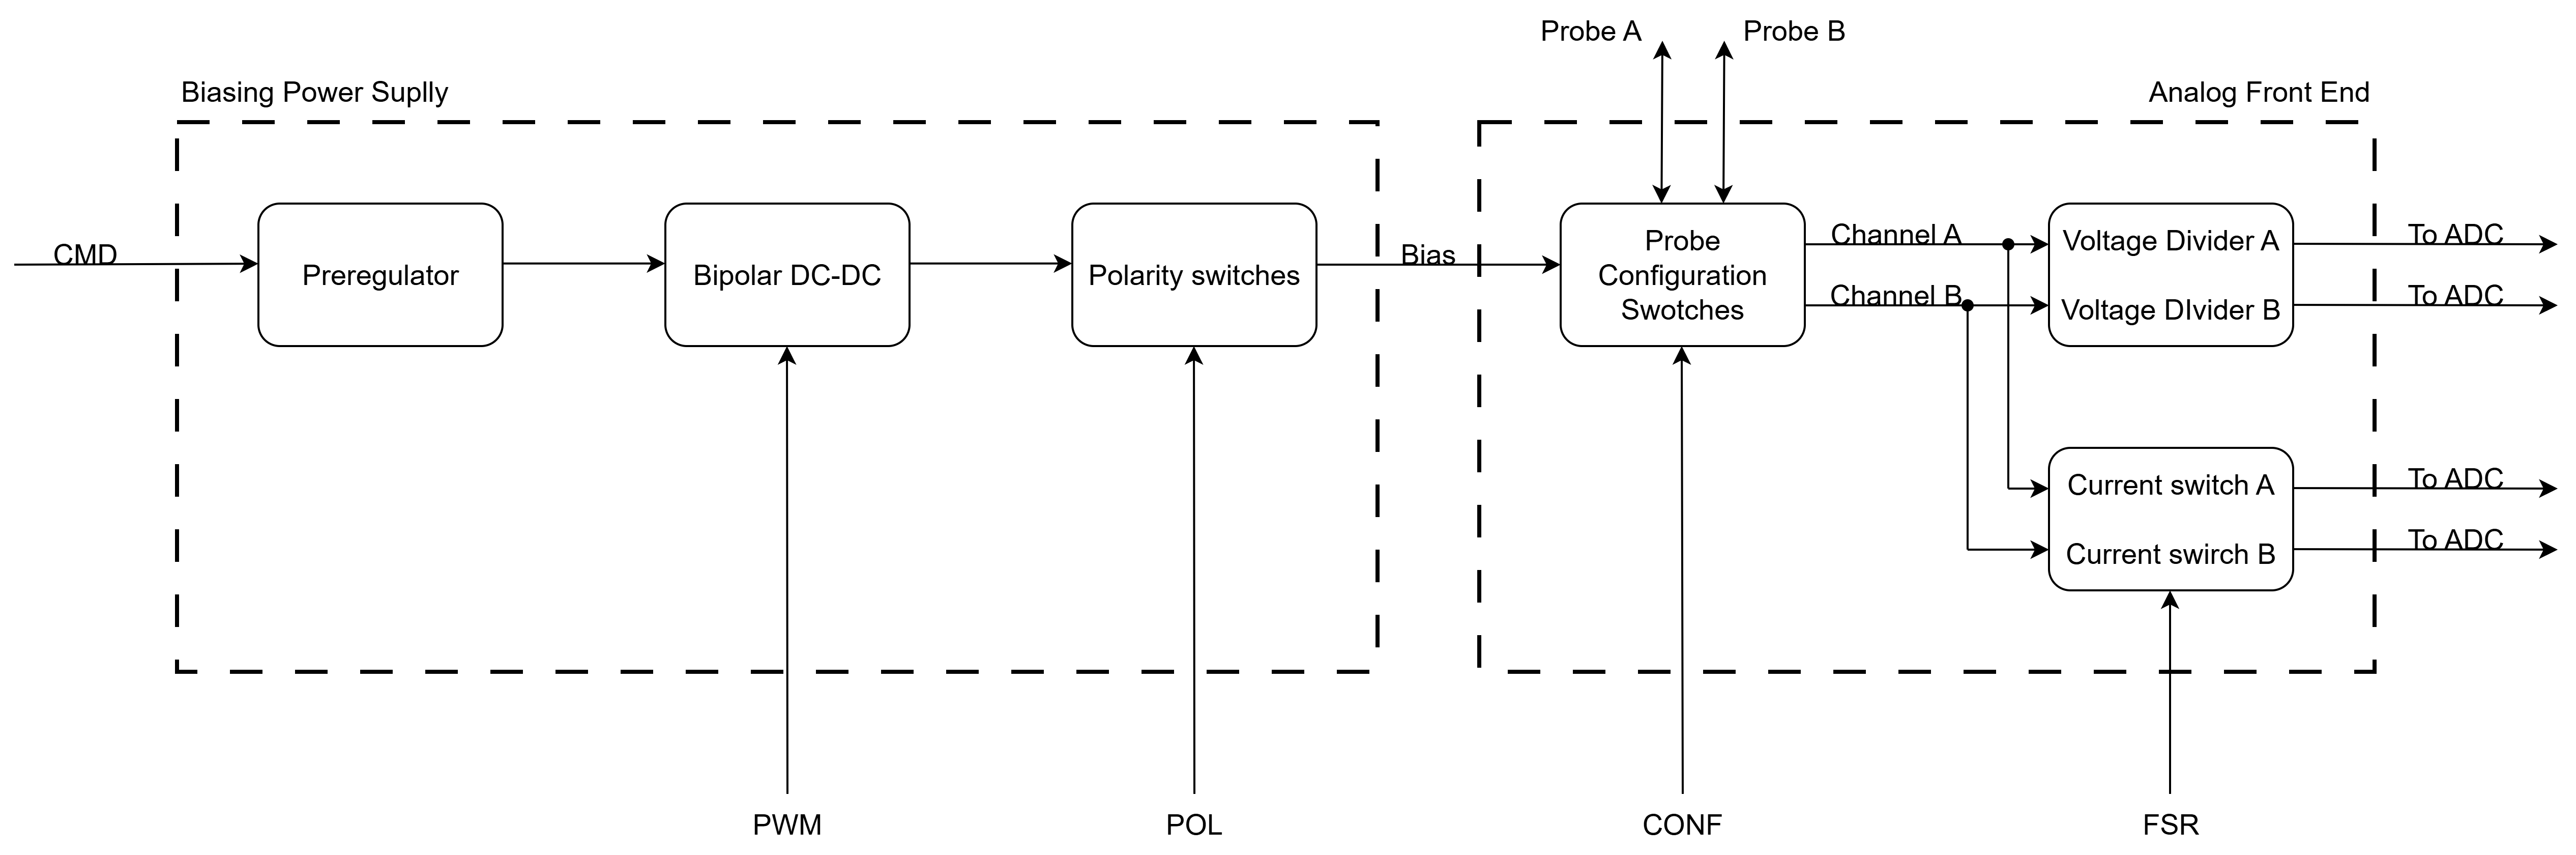
\includegraphics[width=7in]{bps-afe}
	\caption{Block scheme of the integrated BPS and of the analog front-end.}
	\label{fig4}
\end{figure*}



\subsection{Biasing Power Supply}

Conventional COTS power supplies are generally designed for broad laboratory applications, where linear behavior is often a key requirement, and are therefore oversized for Langmuir probe diagnostics, leading to unnecessary cost, complexity, and footprint overhead. In contrast, the electrical requirements of Langmuir probes are dictated by the probe I-V characteristic. In the ion saturation region, where the probe voltage $V_p$ is much smaller than the floating potential $V_f$, relatively high bias voltages are required while probe current remains limited. Conversely, when $V_p > V_f$, that is, when the probe is in the electron retardation region, current increases approximately exponentially whereas the required voltage is comparatively low. Since maximum voltage and maximum current are not required simultaneously, the power delivery stage can be optimized for the effective operating envelope of the diagnostic. Furthermore, strict output linearity is not required; therefore, the linear output stage can be eliminated, reducing the overall footprint and freeing valuable space, but increasing the output control complexity.

The Biasing Power Supply (BPS) adopts a dual-stage output control architecture consisting of a preregulator followed by a bipolar DC-DC converter, as illustrated in Fig.~\ref{fig4}. The preregulator provides slow but high-precision voltage control, whereas the DC-DC stage ensures fast transient response during bias modulation. Output polarity selection is implemented through MOSFET-based switching, allowing the appropriate converter output to be routed to the probe.

Bias waveform generation can be adapted to different measurement scenarios. Although a high-speed communication interface enables real-time waveform updates, closed-loop execution latency may limit performance during high-frequency voltage sweeps. To address this issue, waveform samples can be preloaded into controller memory, reducing communication overhead and enabling deterministic waveform generation.

Furthermore, the architecture allows the integrated BPS to be bypassed and replaced by an external power supply for applications requiring higher power ratings.



\subsection{Analog Front End}

The analog front-end provides the electrical interface between the Langmuir probes and the acquisition electronics. Each module supports two independent probe channels, both equipped with dedicated voltage and current sensing circuits to enable simultaneous acquisition of the probe I-V characteristics, as depicted in Fig.~\ref{fig4}. The module supports a programmable polarization voltage up to \measure{\pm100}{V}, with a maximum drive current of \measure{800}{mA}.

The system supports floating-potential (FP), single-probe (SLP), and double-probe (DLP) measurement configurations. An additional configuration is provided to disconnect the probes from the circuit.

To maximize robustness in electrically noisy environments and to reduce noise propagation, the front-end is implemented exclusively with passive components, avoiding active semiconductor devices. This design choice reduces susceptibility to EMI and improves reliability under harsh electrical conditions.

Measurement range selection and probe configuration are implemented through two switch networks that dynamically select shunt resistors and operating modes without introducing active gain stages. Probe potential measurements are performed using a fixed voltage divider. In addition, dedicated protection circuits are implemented at the input of each acquisition channel to mitigate voltage and current overshoots.



\subsection{Control and Acquisition Unit}

The probe module integrates both an FPGA and a microcontroller, each electrically isolated from the high-voltage bias stage and analog front-end. The FPGA is responsible for time-critical operations, including fast control loops, and protection logic, whereas the microcontroller manages supervisory functions such as module configuration.

Signal acquisition is performed through a \measure{16}{bit} sigma-delta ($\Sigma\Delta$) ADC with programmable sampling frequency, enabling adaptation to different plasma operating conditions. Isolation between the analog and digital domains is achieved directly within the converter. For this application the AD7405 has been used \cite{AD7405}. Effective resolution is declared at 14.2 bit with an oversampling ratio (OSR) of $256$, which corresponds to an effective sampling frequency Fs of 78.125 kHz. The 1-bit modulator operates at a sampling frequency of $f_s = \measure{20}{MHz}$, and the effective output sampling frequency $F_s$ depends on the selected OSR according to
\begin{equation}
	\label{eq:adc_noise}
	F_s = \frac{f_s}{\mathrm{OSR}}.
\end{equation}
Increasing the OSR reduces the in-band quantization noise and therefore improves the effective resolution of the acquisition chain. The quantization noise is shaped towards higher frequencies and subsequently removed by the digital decimation filter. Consequently, larger OSR values provide higher Effective Number of Bits (ENOB) at the expense of a lower output sampling frequency, according to (\ref{eq:adc_noise}), thus introducing a trade-off between measurement bandwidth and effective resolution.



	
	\section{Hardware-Software Integration} \label{secIV}
	The Kria K26 SoM enables tight integration between hardware-programmable logic and embedded software. A Linux-based operating system running on the ARM processing cores manages the interaction between custom FPGA modules and user-space applications, providing a unified framework for data acquisition and control. The hardware–software platform is organized as a multi-layer architecture, comprising bare-metal firmware for low-level hardware management, C/C++ drivers and middleware for system services, and a high-level API that exposes the system functionality to user applications.

The bottom layer consists of the bare-metal firmware running on the FPGA, which implements the fundamental Register Transfer Level (RTL) building blocks, written in Hardware Descriptive Language (HDL), and exposes the memory-mapped registers used for system configuration and control.

The middleware layer provides the coordination and control mechanisms required to manage the execution of system tasks and the communication between lower-level components and the high-level application interface.These functionalities are implemented using the MARTe2 real-time framework, which provides the infrastructure required for deterministic task scheduling, data exchange, and system supervision. Dedicated custom drivers are implemented to access the memory-mapped registers and read data from the FPGA. 

The high-level API constitutes the top layer of the software stack and exposes the system functionalities to the user. It provides a user-oriented interface through a set of high-level functions that enable data management, storage, and post-processing, while abstracting the complexity of the underlying hardware and software layers.




	
	\section{System Validation} \label{secV}
	\begin{table}[t]
	\centering
	\caption{Noise and effective resolution measurements of the acquisition chain.}
	\label{tab:noise_measurements}
	
	\begin{subtable}[t]{0.49\textwidth}
		\centering
		\caption{Voltage noise evaluation.}
		\label{tab:voltage_noise}
		
		\footnotesize
		\renewcommand{\arraystretch}{1.5}
		
		\resizebox{\linewidth}{!}{
			\begin{tabular}{c|c|c|c|c}
				\toprule
				$\mathrm{OSR}$ & $\measure{\mathrm{ENOB}}{[bit]}$ & $\measure{\mathrm{LSB}_{eff}}{[mV]}$ & $\measure{\sigma_m}{[mVrms]}$ & $\measure{V_{off}}{[mV]}$ \\
				\midrule
				
				\multicolumn{5}{c}{\textit{Channel A}} \\
				\midrule
				$128$ & $13.5$ & $36.6$ & $10.60$ & $-196.70$\\
				$256$ & $13.9$ & $28.2$ & $8.15$ & $-196.89$\\
				$512$ & $14.1$ & $23.8$ & $6.87$ & $-196.40$\\
				$1024$ & $14.4$ & $20.2$ & $5.82$ & $-195.90$\\
				
				\midrule
				
				\multicolumn{5}{c}{\textit{Channel B}} \\
				\midrule
				$128$ & $13.5$ & $36.6$ & $10.60$ & $-210.00$\\
				$256$ & $13.8$ & $28.8$ & $8.33$ & $-211.71$\\
				$512$ & $14.1$ & $24.3$ & $7.02$ & $-211.90$\\
				$1024$ & $14.2$ & $21.8$ & $6.28$ & $-212.00$\\
				
				\bottomrule
			\end{tabular}
		}
	\end{subtable}
	
	\vspace{0.5cm}
	
	\begin{subtable}[t]{0.49\textwidth}
		\centering
		\caption{Current noise evaluation.}
		\label{tab:current_noise}
		
		\footnotesize
		\renewcommand{\arraystretch}{1.5}
		\resizebox{\linewidth}{!}{
			\begin{tabular}{c|c|c|c|c}
				\toprule
				$\measure{\mathrm{FSR}}{[mA]}$ & $\measure{\mathrm{ENOB}}{[bit]}$ & $\measure{\mathrm{LSB}_{eff}}{[\mu A]}$ & $\measure{\sigma_m}{[\mu Arms]}$ & $\measure{I_{off}}{[uA]}$ \\
				\midrule
				
				\multicolumn{5}{c}{\textit{Channel A}} \\
				\midrule
				$\pm1.31$ & 13.8 & $0.19$ & $0.05$ & $0.20$\\
				$\pm13.06$ & 14.1 & $1.48$ & $0.43$ & $1.89$\\
				$\pm127.99$ & 14.1 & $14.3$ & $4.12$ & $18.87$\\
				$\pm1281.23$ & 14.0 & $159.08$ & $45.92$ & $177.9$\\
				
				\midrule
				
				\multicolumn{5}{c}{\textit{Channel B}} \\
				\midrule
				$\pm1.31$ & 13.6 & $0.21$ & $0.06$ & $0.03$\\
				$\pm13.06$ & 14.1 & $1.54$ & $0.44$ & $0.01$\\
				$\pm127.99$ & 14.3 & $12.67$ & $3.66$ & $0.34$\\
				$\pm1281.23$ & 13.7 & $188.92$ & $54.54$ & $-6.31$\\
				
				\bottomrule
			\end{tabular}
		}
	\end{subtable}
\end{table}

To assess the functionality and performance of the proposed system, a comprehensive set of tests was conducted. The initial test campaign was aimed at verifying compliance with the requirements listed in Table~\ref{tab:meas_ranges}, whereas subsequent tests were performed to evaluate the system performance and characterize its operational behavior. During this stage, a dedicated test application was used in place of the MARTe2 framework in order to isolate the hardware performance and simplify the validation procedure. In addition, all data analysis and parameter extraction were performed offline after the acquisition stage.


\subsection{Noise, Resolution \& Offsets Evaluation} \label{subsecVA}

\begin{figure*}[t]
	\centering
	\subfloat[Floating potential measurement in FP configuration]{
		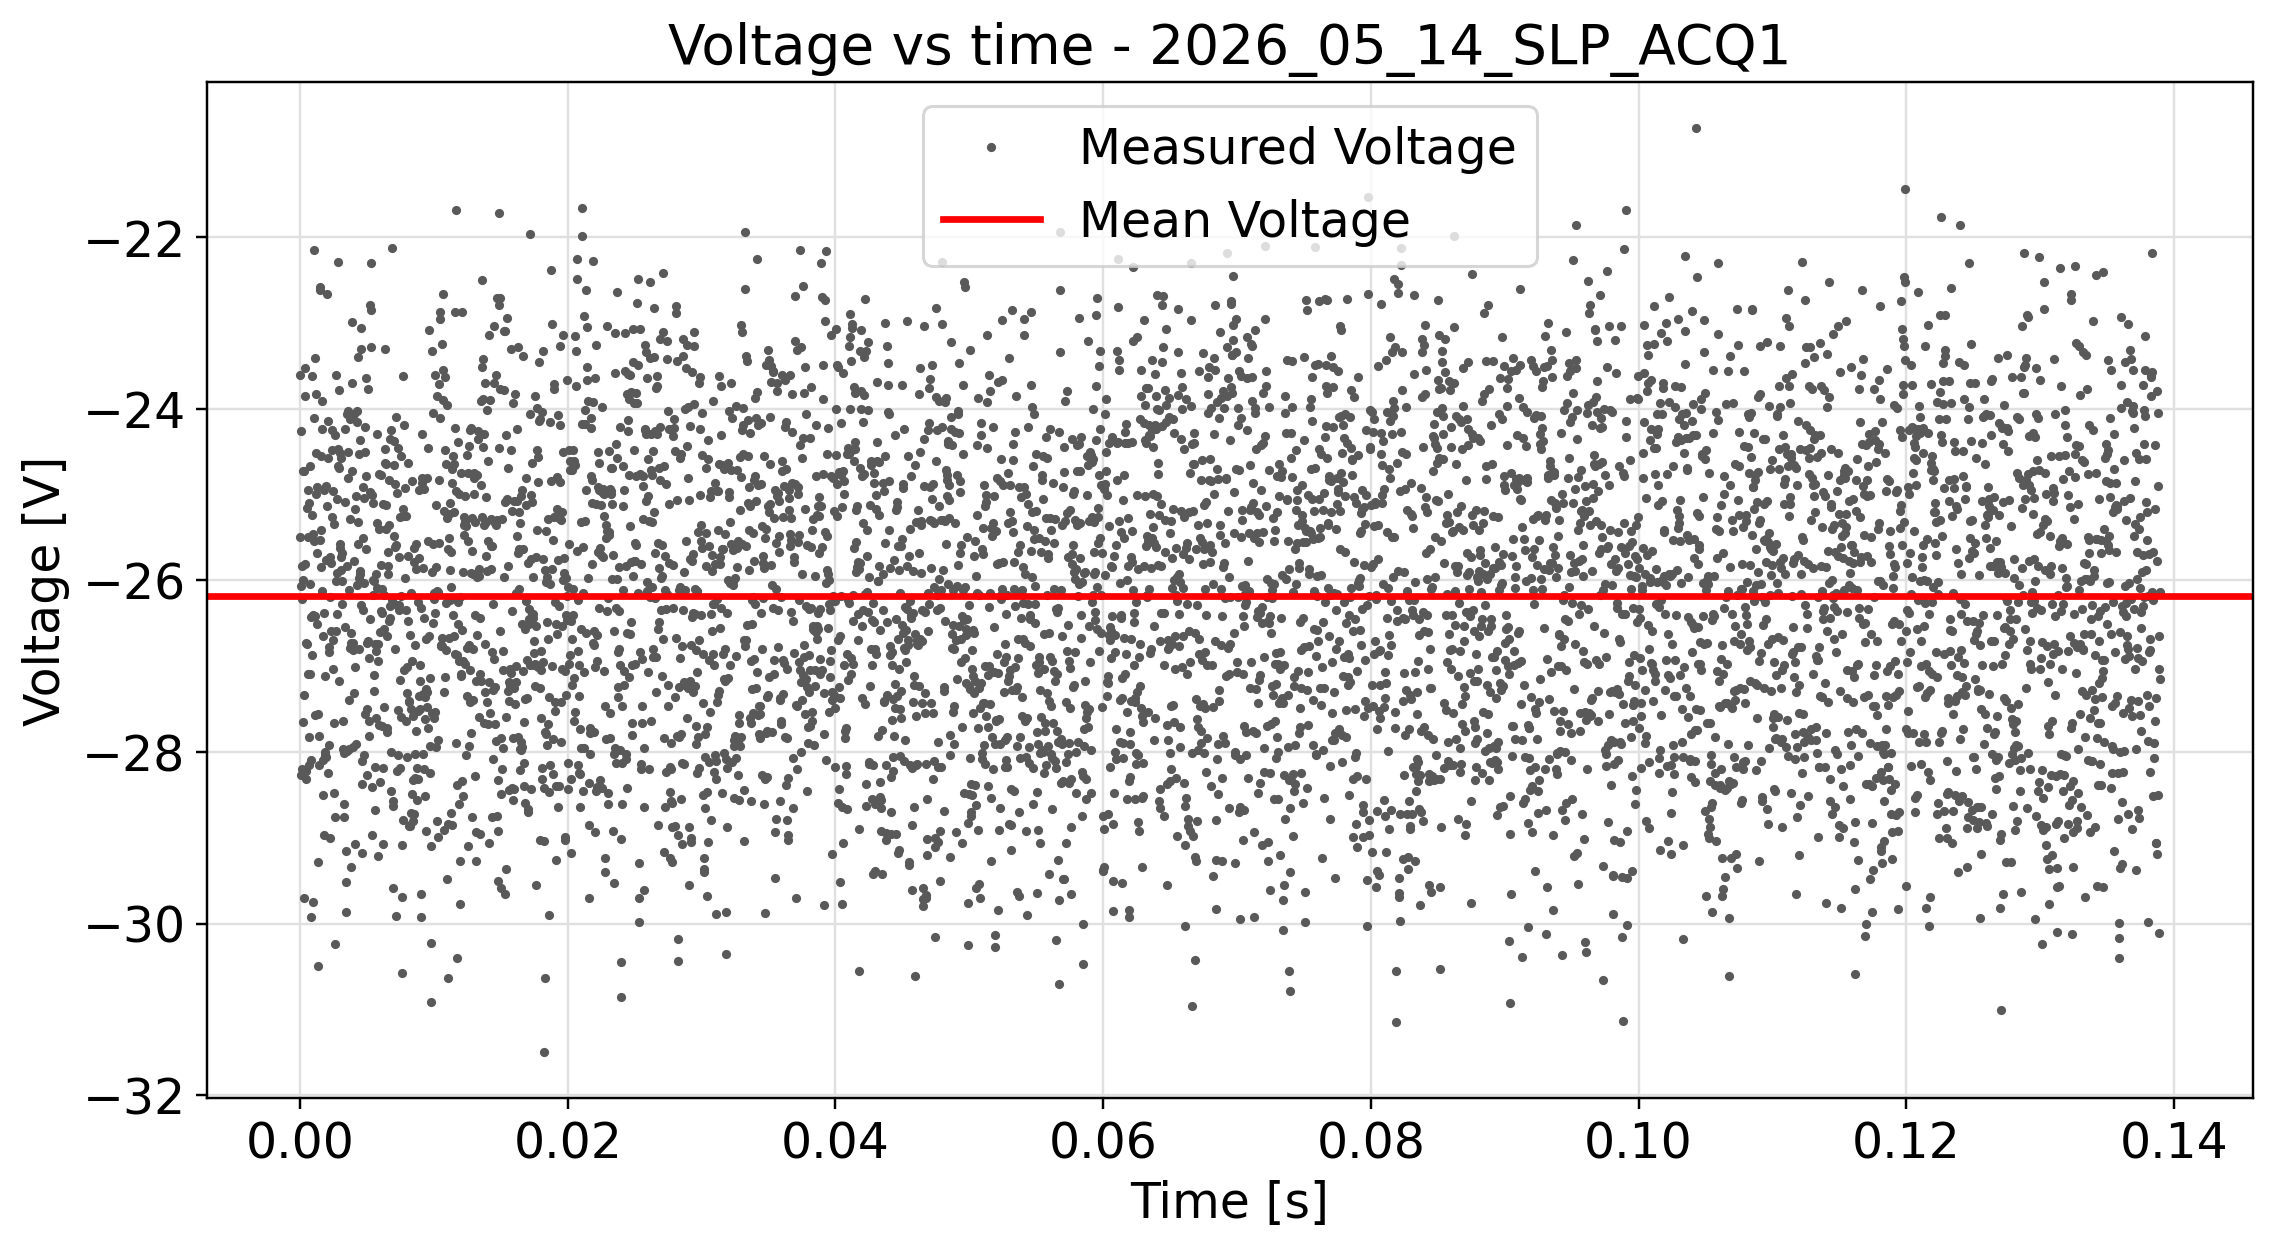
\includegraphics[width=3.4in]{2026_05_14_SLP_ACQ1_voltage_time}
		\label{fig5a}
	}
	\hfill
	\subfloat[SLP characteristic. The plot shows the four-parameter fit (red line) and the plasma parameters extracted from the measurement.]{
		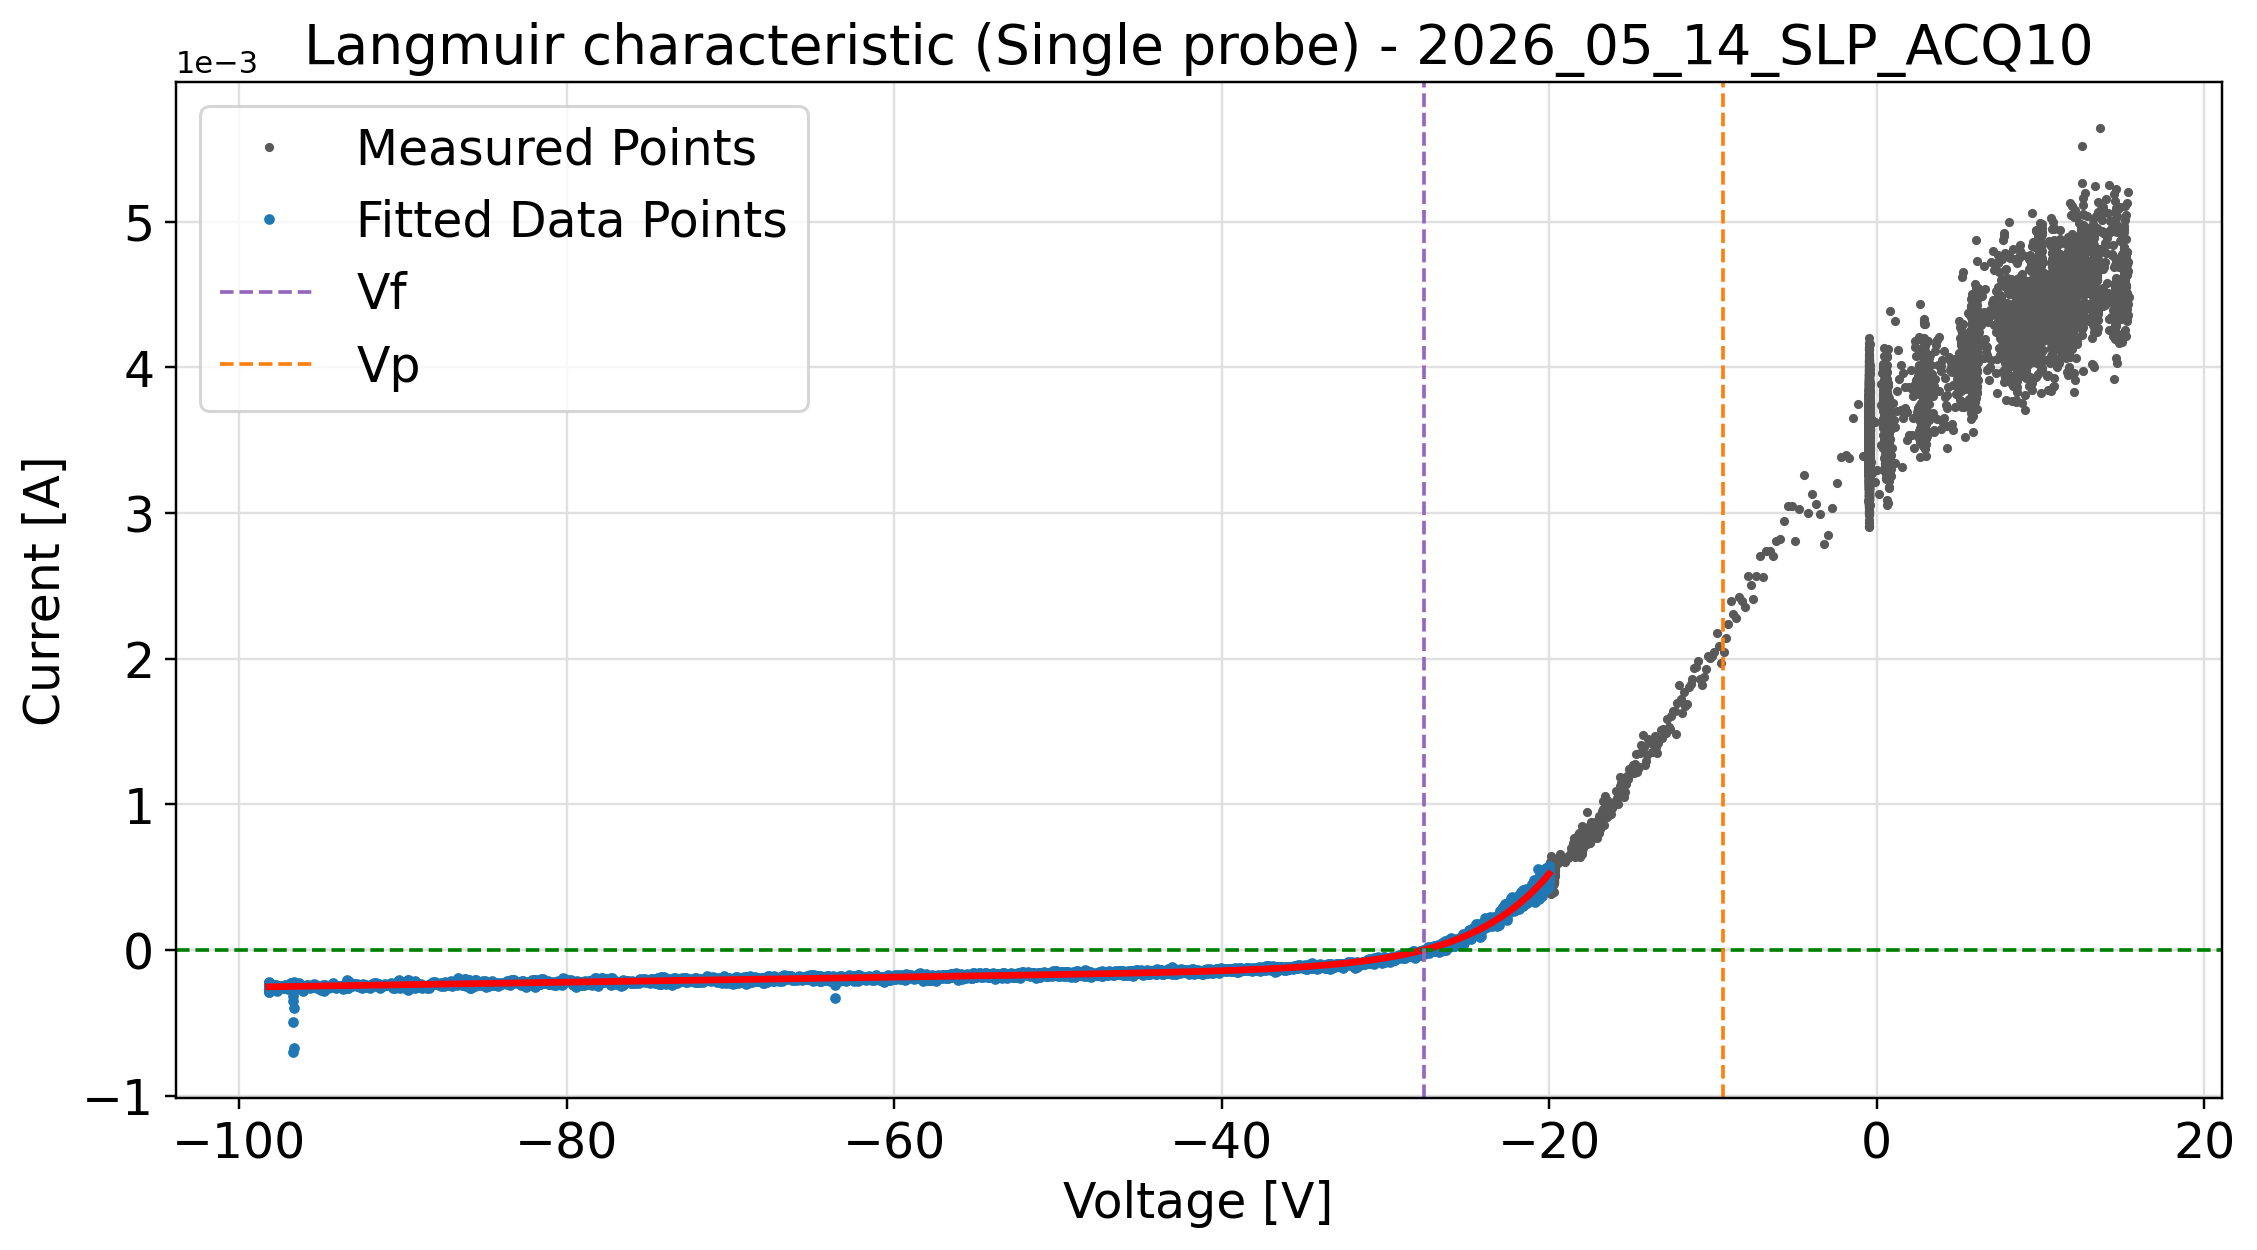
\includegraphics[width=3.4in]{2026_05_14_SLP_ACQ10_fits}
		\label{fig5b}
	}
	
	\caption{Representative floating-potential acquisition and SLP characteristic obtained during EPICA evaluation.}
	\label{fig5}
\end{figure*}

Several parameters were evaluated to quantify the performance of the acquisition chain. For both the voltage and current acquisition channels, the ENOB, the residual rms noise $\sigma_m$, the effective quantization step $\mathrm{LSB}_{eff}$, and the mean value $\mu_m$, representing the channel offset, were measured. The parameter $\sigma_m$ represents the residual noise floor of the acquisition chain, whereas $\mathrm{LSB}_{eff}$ corresponds to the effective resolution associated with the measured noise level. The ENOB can be estimated from the measured rms noise by considering the quantization error of an ideal analog-to-digital converter. The quantization error is uniformly distributed within the interval $\left[-\mathrm{LSB}_{eff}/2, +\mathrm{LSB}_{eff}/2\right]$ therefore, its standard deviation is
\begin{equation}
	\sigma_q = \frac{\mathrm{LSB}_{eff}}{\sqrt{12}}.
	\label{eq:ENOB1}
\end{equation}
By equating the measured rms noise $\sigma_m$ to the equivalent quantization noise, the effective resolution can be expressed as
\begin{equation}
	\mathrm{ENOB} = \log_2\left(\frac{\mathrm{FSR}}{\sigma_{m}\sqrt{12}}\right),
	\label{eq:ENOB2}
\end{equation}
where FSR denotes the full-scale range of the acquisition channel, LSB the nominal Least Significant Bit, and $\mathrm{LSB}_{eff}$ the effective quantization step corresponding to the measured noise floor. The corresponding nominal and effective quantization steps are
\begin{equation}
	\mathrm{LSB} = \frac{\mathrm{FSR}}{2^{16}}, \qquad \mathrm{LSB}_{eff} = \frac{\mathrm{FSR}}{2^{\mathrm{ENOB}}}.
	\label{eq:ENOB3}
\end{equation}

The voltage noise performance was evaluated with the integrated BPS disconnected from the probe circuitry by configuring both channels in FP mode. By configuring the system in FP mode, noise contributions from the BPS are excluded from the measurement, allowing the performance of the analog front-end and ADC acquisition chain to be evaluated independently. The inputs were subsequently short-circuited in order to eliminate external noise sources. ENOB and effective resolution values, computed using (\ref{eq:ENOB1}) and (\ref{eq:ENOB3}), are summarized in Table~\ref{tab:voltage_noise}. The voltage acquisition chain has a nominal full-scale range of $\mathrm{FSR}=\measure{423.03}{V}$, corresponding to a nominal quantization step of $\mathrm{LSB}=\measure{6.455}{mV}$, which is equal for each voltage channel. The nominal FSR differs from the value reported in Table~\ref{tab:meas_ranges} due to the voltage-divider ratio adopted in the acquisition chain. This design choice was made to preserve the capability of measuring higher voltages when external bias supplies are used in place of the integrated BPS. Table \ref{tab:voltage_noise} summarizes the measured noise and effective resolution values.

Current measurement validation was performed by configuring the probe module in the SLP operating mode and applying an external fixed bias voltage for each current FSR. This approach was adopted to ensure that noise contributions associated with the integrated BPS were excluded from the evaluation of the acquisition chain performance. During these tests, the acquisition frequency was fixed at $F_s=\measure{78.125}{kHz}$.

Evaluation of the offsets ($V_{off}$ and $I_{off}$) related to each channel and FSR was carried out applying the same procedure of the current noise evaluation, physically detaching the integrated BPS and short circuiting the BPS rails of the analog front-end and the inputs.



\subsection{Probe Characteristic} \label{subsecVB}

Characterization of the overall system behavior was carried out using a dedicated vacuum chamber capable of generating low-temperature plasmas. Plasma operating conditions were controlled through adjustments of the gas pressure and electrode bias voltage, thereby enabling the generation of different plasma regimes. 

Plasma parameters were estimated by fitting the acquired I-V characteristics using the four-parameter model
\begin{equation}
	I(V)=I_s\left[1+R(V-V_f)\right] \left(e^{\frac{V-V_f}{T_e}}-1\right),
	\label{eq:model_slp}
\end{equation}
where $T_e$ is the electron temperature, $I_s$ the ion saturation current, $V_f$ the floating potential, and $R$ a linear correction factor accounting for deviations from the ideal ion saturation regime. Once the fitting parameters $(T_e, I_s, V_f, \mathrm{R})$ were obtained, $N_e$ and $V_p$ were estimated from the fitted floating potential and electron temperature according to the classical Langmuir probe theory \cite{Chen}. A preliminary acquisition was performed in the FP configuration to determine the probe floating potential. The corresponding measurement is shown in Fig.~\ref{fig5a}. Unlike the noise characterization tests described in Section~\ref{subsecVA}, the measured fluctuations in this case include contributions from both the acquisition chain and the plasma itself. Consequently, the observed noise level is significantly higher than the intrinsic noise floor of the instrumentation. The FP measurement yielded a mean floating potential of $V_f=\measure{-26.2}{V}$ and an RMS fluctuation level of $\sigma_m=\measure{1.81}{Vrms}$. Subsequently, the system was operated in the SLP configuration to acquire the complete I-V characteristic. A representative characteristic obtained from a helium plasma is shown in Fig.~\ref{fig5b}. The corresponding plasma parameters are reported in Table \ref{tab:SLP}.

Whereas the FP and SLP configurations were successfully tested using the plasma source, validation of the DLP configuration was limited by the inability to place two probes in regions characterized by sufficiently uniform plasma conditions. Therefore, a dummy load comprising a resistor and two anti-series Zener diodes was connected to the probe module. This setup was used to verify the correct operation of the front-end switching network and the associated acquisition circuitry under DLP conditions. The resulting I-V characteristic is shown in Fig.~\ref{fig6}

\begin{figure}[t]
	\centering
	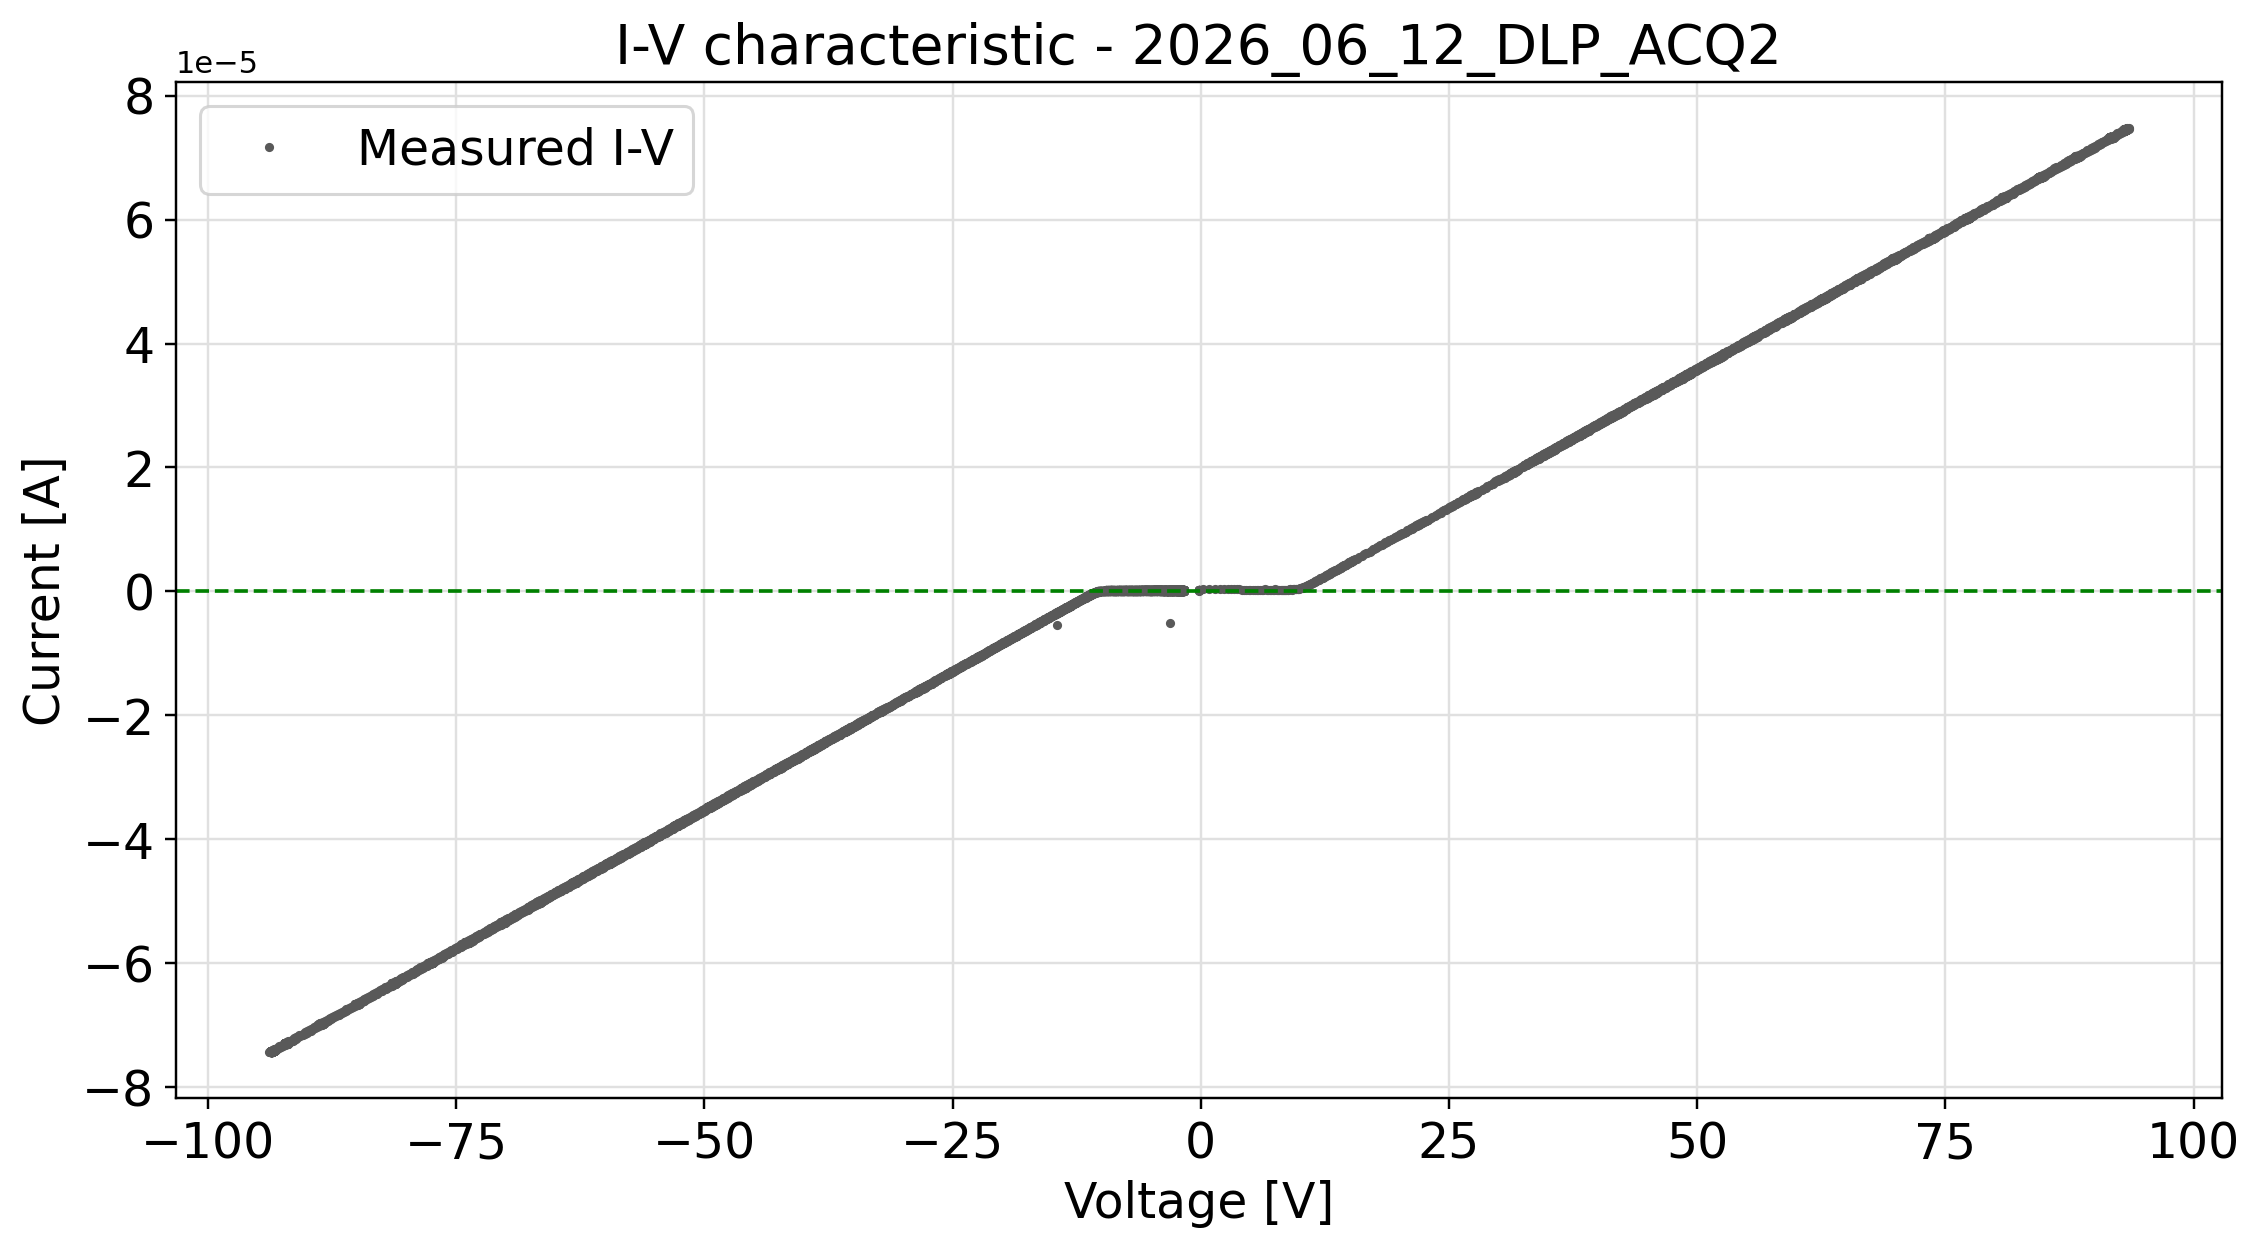
\includegraphics[width=3.4in]{2026_06_12_DLP_ACQ2_i-v}
	\caption{Functional verification of the DLP configuration using a dummy load composed of anti-series Zener diodes. Acquisition performed at $F_s = \measure{78.125}{kHz}$ and $\mathrm{FSR} = \measure{\pm1}{mA}$.}
	\label{fig6}
\end{figure}

\begin{table}[t]
	\centering
	\footnotesize
	\renewcommand{\arraystretch}{1.5}
	\caption{Plasma parameters extrapolated from the SLP characteristics.}
	\label{tab:SLP}
	
	\begin{tabular}{c|c|c|c|c}
		\toprule
		$\measure{T_e}{[eV]}$ & $\measure{I_s}{[A]}$ & $\measure{V_f}{[V]}$ & $\measure{V_p}{[V]}$ & $\measure{N_e}{[m^{-3}]}$\\
		\midrule
		$4.53$ & $1.31\cdot10^{-4}$ & $-27.7$ & $-9.39$ & $7.82\cdot10^{16}$\\
		\bottomrule
	\end{tabular}
	
\end{table}

	
	\section{Results Discussion} \label{secVI}
	
\begin{figure*}[t]
	\centering
	\subfloat[Voltage plateau and subsequent voltage jump when the condition $|V_{\mathrm{probe}}| \leq |V_f|$ is met.]{
		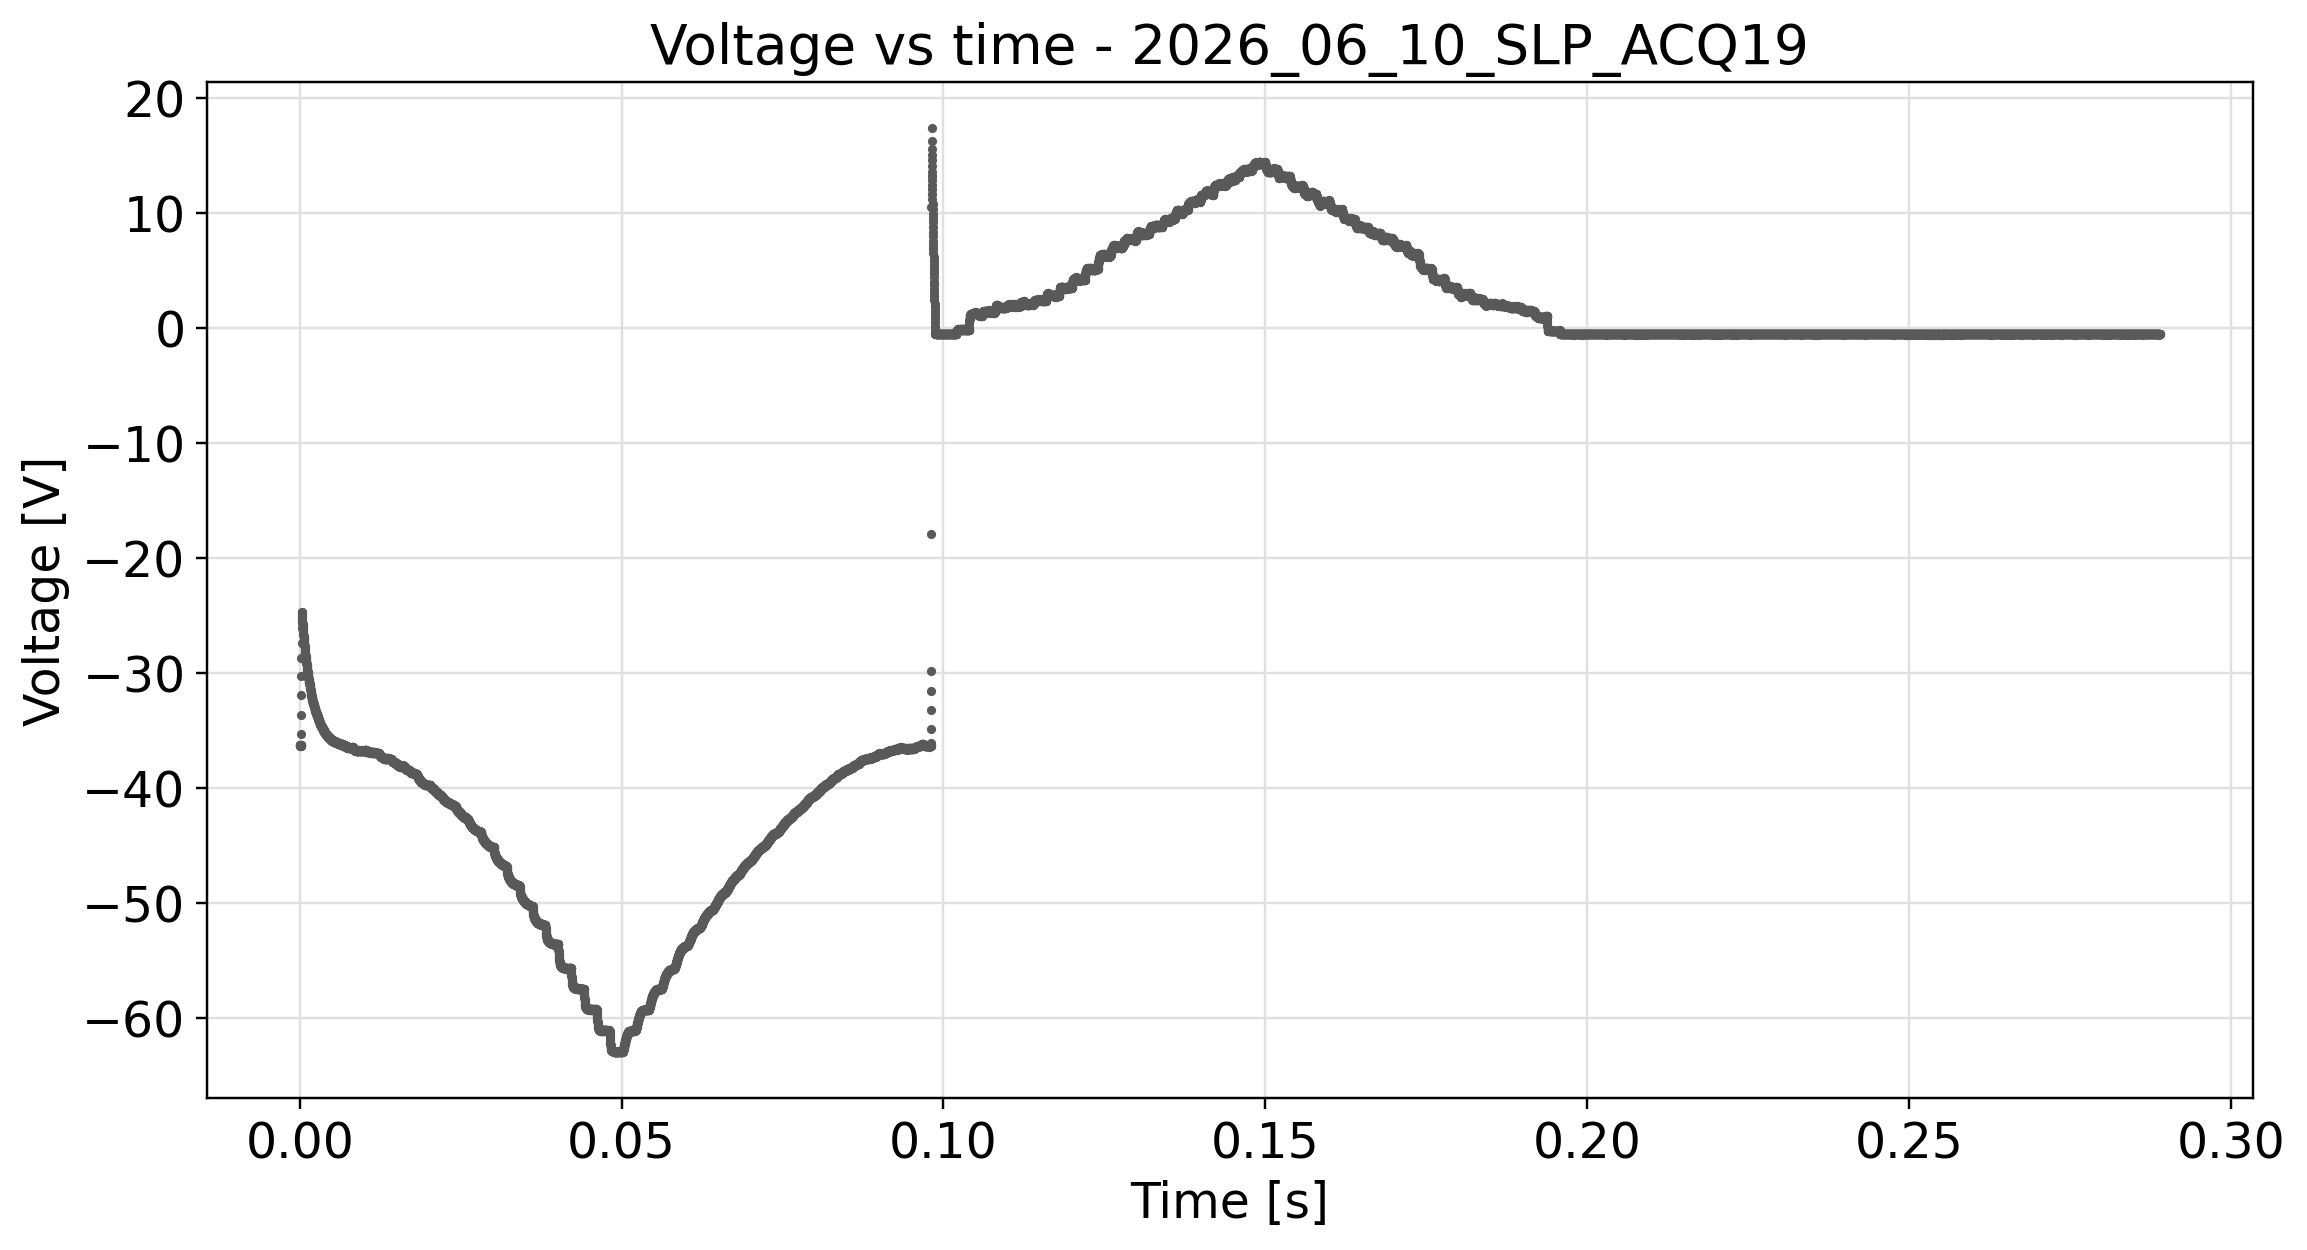
\includegraphics[width=3.4in]{2026_06_10_SLP_ACQ19_voltage_time}
		\label{fig7a}
	}
	\hfill
	\subfloat[Effect on the I-V characteristics.]{
		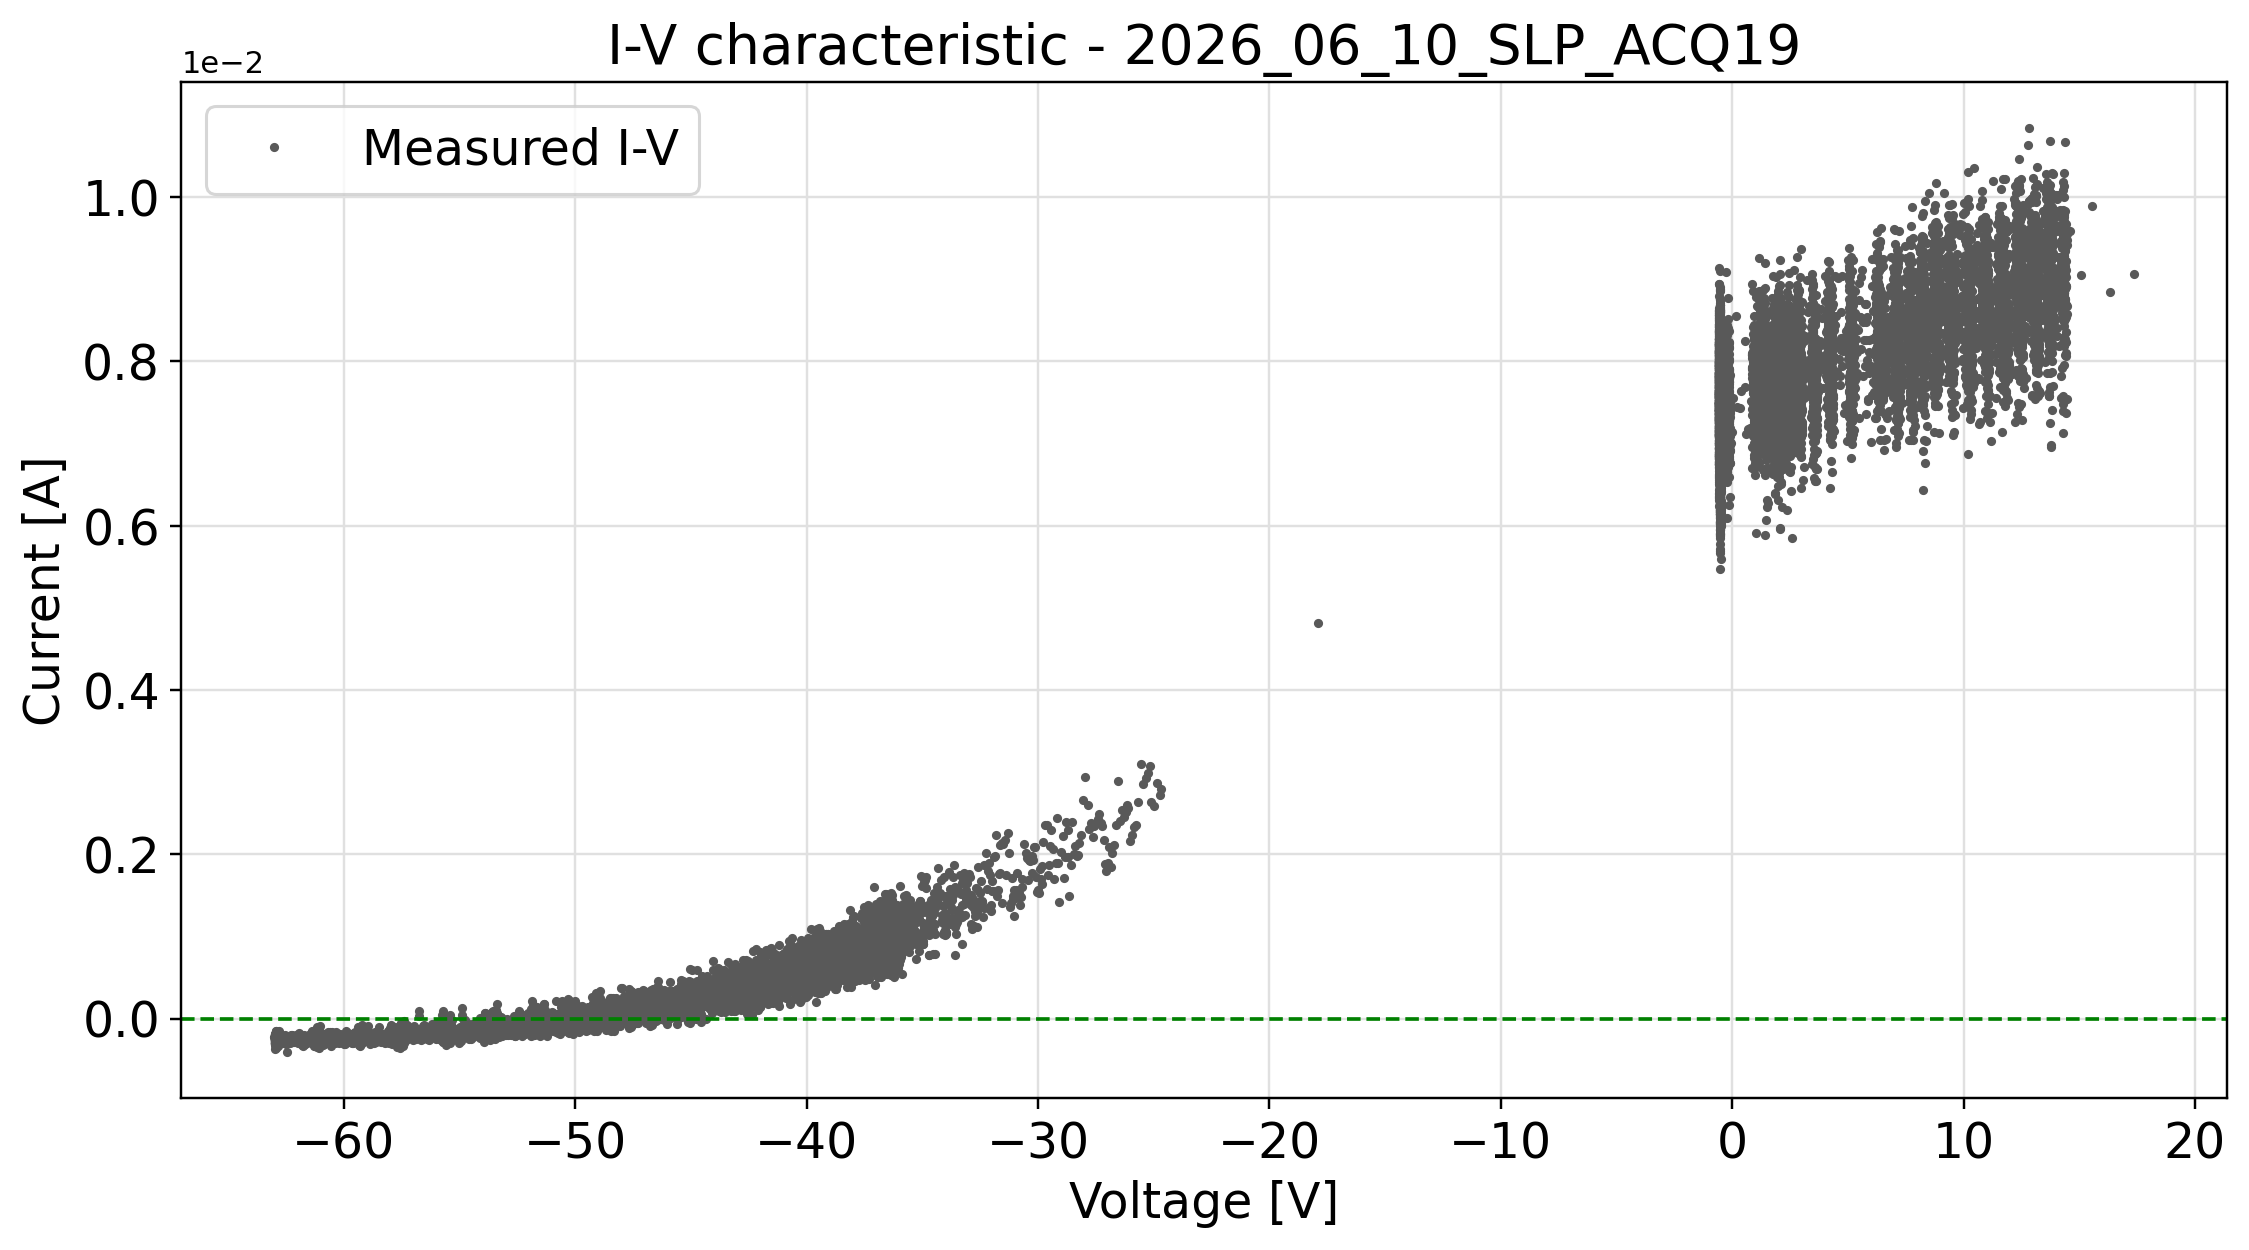
\includegraphics[width=3.4in]{2026_06_10_SLP_ACQ19_i-v}
		\label{fig7b}
	}
	
	\caption{Acquisition of a high-density plasma.}
	\label{fig7}
\end{figure*}

The results reported in Table~\ref{tab:noise_measurements} demonstrate the expected trade-off between acquisition bandwidth and effective resolution inherent to $\Sigma\Delta$ conversion architectures. For the voltage acquisition chain, the ENOB increases from approximately $\measure{13.5}{bit}$ at $\mathrm{OSR}=128$ to $\measure{14.4}{bit}$ at $\mathrm{OSR}=1024$. The nominal operating condition was selected at $\mathrm{OSR}=256$, corresponding to an output sampling frequency of $\measure{78.125}{kHz}$. Under these conditions, the measured ENOB is $\measure{13.9}{bit}$ and $\measure{13.8}{bit}$ for Channel~A and Channel~B, respectively. These values are slightly lower than the $\measure{14.2}{bit}$ specified in the AD7405 datasheet. This difference is expected, since the datasheet value primarily characterizes the converter itself under controlled test conditions, whereas the measurements reported here include the complete acquisition chain. In particular, the analog front-end, ADC, and power supply circuitry share a common ground reference, making the measured noise representative of the integrated system rather than of the converter alone. The measured residual noise remains below the maximum value specified in Table~\ref{tab:meas_ranges}, confirming compliance with the voltage acquisition requirements defined for MITICA operation.

The current acquisition results reported in Table~\ref{tab:noise_measurements} demonstrate stable performance across more than three decades of full-scale range. Unlike the voltage acquisition chain, the current measurements were all performed at the nominal operating condition of $\mathrm{OSR}=256$. Under these conditions, the measured ENOB remains close to $\measure{14}{bit}$ for all acquisition ranges, indicating that the programmable shunt selection network introduces negligible degradation of the overall acquisition performance. The measured noise scales consistently with the selected current range, ranging from approximately $\measure{0.05}{\mu A_{rms}}$ for the $\pm\measure{1.31}{mA}$ range up to $\measure{45.92}{\mu A_{rms}}$ for the $\pm\measure{1.28}{A}$ range. Comparison with the requirements listed in Table~\ref{tab:meas_ranges} shows that all investigated current ranges satisfy the specified noise limits. In particular, the $\measure{\pm1}{mA}$ and $\measure{\pm10}{mA}$ ranges exhibit noise levels significantly lower than the required thresholds, while the $\pm\measure{100}{mA}$ and $\pm\measure{1}{A}$ ranges remain comfortably within the corresponding limits. These results demonstrate that the proposed acquisition architecture preserves adequate measurement resolution over the entire operating range foreseen for MITICA.

The offset measurements reported in Table~\ref{tab:noise_measurements} show a systematic voltage offset of approximately \measure{200}{mV} for both acquisition channels. The similarity of the measured values suggests that the offset originates from common elements of the analog front-end rather than from channel-specific effects. Although significantly larger than the measured noise floor, the offset corresponds to less than $0.05\%$ of the acquisition full-scale range ($\mathrm{FSR}=\measure{423.03}{V}$) and can therefore be considered negligible for the intended application. Furthermore, the systematic nature of the offset allows straightforward software compensation during normal operation. Current offsets exhibit an approximately proportional dependence on the selected measurement range and remain comparable to the corresponding effective quantization step. Even in the worst-case condition, the measured offset remains
well below the associated full-scale range and does not affect compliance with the requirements listed in Table~\ref{tab:meas_ranges}. Consequently, the contribution of offset-related errors to the overall measurement uncertainty is negligible with respect to the required diagnostic accuracy.

The plasma characterization results further validate the capability of the proposed system to perform complete Langmuir probe measurements under realistic operating conditions. The characteristic reported in Fig.~\ref{fig5b} exhibits the expected transition between the ion saturation, electron retardation, and electron saturation regions, indicating the correct operation of both the probe polarization stage and the acquisition chain. The agreement between the measured characteristic and the fitted model demonstrates that the acquisition system provides sufficient resolution and dynamic range to support reliable extraction of plasma parameters. This result validates not only the performance of the individual acquisition channels but also the correct integration of the polarization, conditioning, acquisition, and processing stages within the module.

During the experimental campaign, a limitation of the present bias generation implementation was identified. Whenever the generated probe voltage satisfies the condition $|V_{\mathrm{probe}}| \leq |V_f|$, the output remains clamped to the floating potential and does not continuously reach $\measure{0}{V}$, as illustrated in Fig.~\ref{fig7a}. As a consequence, a discontinuity in the I-V characteristic is introduced when the output polarity changes, transitioning from $V_f$ to $\measure{0}{V}$, as seen in Fig.~\ref{fig7b}. The impact of this effect depends on the plasma operating conditions. For low-density plasmas, the slower response of the probe current allows a sufficient number of samples to be acquired within the electron retardation region, enabling reliable reconstruction of the I--V characteristic. Conversely, higher-density plasmas exhibit a significantly faster response, reducing the number of acquired samples around the transition region and producing a discontinuity in the measured characteristic. The identified limitation was subsequently mitigated by modifying the control strategy of the polarity-selection transistors. Instead of operating exclusively as switching devices in fully ON and OFF states, the transistors were driven within their active region, enabling a smoother transition between voltage polarities and eliminating the discontinuity observed around the floating potential.

Although plasma characterization using the DLP configuration was not possible with the available experimental setup, functional verification confirmed the correct operation of the switching network and associated acquisition circuitry.

Overall, the experimental results demonstrate that the proposed architecture provides sufficient measurement performance to support both plasma characterization and large-scale Langmuir probe deployments.
	
	\section{Conclusion} \label{secVII}
	This work presented EPICA, an integrated platform for Langmuir probe diagnostics that combines probe bias generation, signal conditioning, data acquisition, and embedded processing within a modular architecture. The system was specifically developed to address the scalability challenges associated with large Langmuir probe arrays, such as those foreseen for MITICA.

Experimental validation confirmed compliance with the measurement requirements defined for MITICA operation. The proposed architecture successfully demonstrated high-resolution voltage and current acquisition and the capability to perform complete Langmuir probe measurements.

Unlike conventional implementations based on centralized laboratory instrumentation, EPICA integrates the complete measurement chain within each probe module, significantly reducing wiring complexity, footprint, and system-level integration effort. The combination of distributed bias generation, FPGA-based processing, and compatibility with ITER CODAC provides a scalable solution for large plasma diagnostic systems.

The modular organization of the platform enables straightforward scaling towards the 212 measurement points foreseen for MITICA while preserving synchronization, centralized supervision, and measurement performance.

Future developments will focus on the deployment of the complete MARTe2 software framework and on extended validation of the proposed architecture in ongoing plasma experiments. These activities will provide further assessment of the system performance under realistic operating conditions and support future large-scale deployments.
	
	% \section*{References}
	\begin{thebibliography}{00}
	\bibitem{Chen} F. F. Chen, ``Langmuir probe diagnostics,'' in \textit{Proc. IEEE-ICOPS Meeting}, Jeju, Korea, 2003.
	
	\bibitem{Crowley} B. Crowley \textit{et al.}, ``Measurement of the electron energy distribution function by a Langmuir probe in an ITER-like hydrogen negative ion source,'' \textit{Nucl. Fusion}, vol.~46, no.~6, pp.~S307--S312, 2006, doi: 10.1088/0029-5515/46/6/S07.
	
	\bibitem{NI} National Instruments, "CompactDAQ Measurement Bundles," NI, Austin, TX, USA. [Online]. Available: \url{https://www.ni.com/en/shop/compactdaq/compactdaq-measurement-bundles.html}.
	
	\bibitem{CAEN} CAEN S.p.A., "Digitizer Families," CAEN – Tools for Discovery. [Online]. Available: \url{https://www.caen.it/sections/digitizer-families/}. 
	
	\bibitem{Kepco} Kepco Inc., "BOP-HV Series High Voltage Bipolar Operational Power Supplies." [Online]. Available: \url{https://www.kepcopower.com/bophv.htm}. 
	
	\bibitem{Toigo} V. Toigo \textit{et al.}, ``The PRIMA test facility: SPIDER and MITICA test-beds for ITER neutral beam injectors,'' \textit{New J. Phys.}, vol.~19, no.~8, p.~085004, Aug. 2017, doi: 10.1088/1367-2630/aa78e8.
	
	\bibitem{SPAGNOLO} SPAGNOLO, Silvia, et al. Final design of electrostatic probes for MITICA beam line components. Fusion Engineering and Design, 2021, 166: 112265.
	
	\bibitem{Ryan} P. J. Ryan, S. D. Elmore, J. R. Harrison, J. Lovell, and R. Stephen, “Overview of the Langmuir probe system on the Mega Ampere Spherical Tokamak (MAST) Upgrade,” Rev. Sci. Instrum., 2024.
	
	\bibitem{KRIA} AMD/Xilinx, ``Kria K26 SOM data sheet,'' AMD, [Online]. Available: \url{https://docs.amd.com/r/en-US/ds987-k26-som/Overview}. 
	
	\bibitem{manduchi} MANDUCHI, G., et al. MARTe2 and MDSplus integration for a comprehensive fast control and data acquisition system. Fusion Engineering and Design, 2020, 161: 111892.
	
	\bibitem{AD7405} Analog Devices, Inc., "AD7405: Isolated Sigma-Delta Modulator with Digital Filter," Rev. B, Norwood, MA, USA. [Online]. Available: \url{https://www.analog.com/media/en/technical-documentation/data-sheets/ad7405.pdf}. 
	
\end{thebibliography}
	
\end{document}